% % % % % % % %  MDT UFSM 2015  % % % % % % % % 
%% Arquivo base para o documento - ver. 1.08 %%
% % % % % % % % % % % % % % % % % % % % % % % % 


% % % OPCOES DE COMPILACAO
% % % PAGINACAO
% % % PAGINACAO SIMPLES (FRENTE): PARA TRABALHOS COM MENOS DE 100 PAGINAS
\documentclass[oneside,openright,12pt]{ufsm_2015} %%%%% OPCAO PADRAO -> PAGINACAO SIMPLES. PARA TRABALHOS COM MAIS DE 100 PAGINAS COMENTE ESTA LINHA E DESCOMENTE A LINHA 
% % % % % % % % % % % % % % % % % % % % % % % % % % % % % % % % % % % % % % %
% PAGINACAO DUPLA (FRENTE E VERSO): PARA TRABALHOS COM MAIS DE 100 PAGINAS
% \documentclass[twoside,openright,12pt]{ufsm_2015}  %%%% PARA TRABALHOS COM MAIS DE 100 PAGINAS DESCOMENTE AQUI
% % % % % % % % % % % % % % % % % % % % % % % % % % % % % % % % % % % % %




% % % %  CODIFICACAO DO TEXTO 
% % % %  POR PADRAO USA-SE UTF8. PARA APLICAR A CODIFICACAO OESTE EUROPEU (ISO 8859-1) DESCOMENTE A LINHA ABAIXO. ELA ATIVA A OPCAO "latin1" DO PACOTE "inputenc"
% \oesteeuropeu
% % % % % % % % % % % 



% % % % % % % % PACOTES PESSOAIS % % % % % % % %  
\usepackage{lipsum}
\usepackage{listings}
%LISTINGS FORMATAÇÃo


%define Javascript language
\lstdefinelanguage{JavaScript}{
keywords={typeof, new, true, false, catch, function, return, null, catch, switch, var, if, in, while, do, else, case, break, out, body, geocodeArea, way, are},
keywordstyle=\color{black}\bfseries,
ndkeywords={class, export, boolean, throw, implements, import, this},
ndkeywordstyle=\color{darkgray}\ttfamily,
identifierstyle=\color{black},
sensitive=false,
commentstyle=\color{purple}\ttfamily,
stringstyle=\color{gray}\ttfamily,
%morestring=[b]',
%morestring=[b]"
}
 
\lstset{
language=JavaScript,
extendedchars=true,
basicstyle=\ttfamily,
showstringspaces=false,
showspaces=false,
numbers=left,
numberstyle=\footnotesize,
numbersep=9pt,
tabsize=2,
breaklines=true,
showtabs=false,
captionpos=t
}


% % % % % % % % DEFINICOES PESSOAIS % % % % % % % %

\usepackage{subfigure}
\usepackage{graphicx}



% % % % % % % % % % % % % % % % % % % % % % % % % % % % % % % % % % % % % % % % % % % 




% % % % % % % % % % % % % % % % % % % % % % % % % % % % % % % % % 
% % % % % % % % % % % % DADOS DO TRABALHO % % % % % % % % % % % % 
% % % % % % % % % % % % % % % % % % % % % % % % % % % % % % % % % 

% % % % % % % % % % INFORMACOES INSTITUCIONAIS % % % % % % % % % % 


% % CENTRO DE ENSINO DA UFSM
\centroensino{Centro de Tecnologia}  %%% NOME POR EXTENSO
\centroensinosigla{CT}  %%% SIGLA

% % CURSO DA UFSM
\nivelensino{Graduação}  %%%%%%% NIVEL DE ENSINO 
\curso{Ciência da Computação}   %%%%% NOME POR EXTENSO
%\ppg{PPGALGO}   %%%%%% SIGLA
\statuscurso{Curso}  %%%% STATUS= {Programa} ou {Curso}
% \EAD  %%%% para cursos EAD
% % % %  LOCAL DO CAMPUS OU POLO
\cidade{Santa Maria}
\estado{RS}


% % % % % % % % % % INFORMACOES DO AUTOR % % % % % % % % % % 
\author{Elmo Santos da Silva Neto}   %%%%% AUTOR DO TRABALHO
\sexo{M} %%%% SEXO DO AUTOR -> M=masculino   F=feminino (IMPORTANTE PARA AJUSTAR PAGINAS PRE-TEXTUAIS)
\grauensino{Bacharelado}    %%%%%%%% GRAU DE ENSINO A SER CONCLUIDO
\grauobtido{Bacharel}    %%%%% TITULO OBTIDO
\email{elmo@inf.ufsm.br}   %%%% E-MAIL PARA CATALOGRAFICA (COPYRIGHT) - OBRIGATORIO
\endereco{Avenida Roraima, nº 1000} %%%% TELEFONE PARA CATALOGRAFICA (COPYRIGHT) (CAMPO OPICIONAL -- CASO NAO POSSUA OU NAO QUEIRA DIVULGAR COMENTE A LINHA)
%\fone{11 2222 3333}   %%%% TELEFONE PARA CATALOGRAFICA (COPYRIGHT) FORMATO {11 2222 3333} (CAMPO OPICIONAL -- CASO NAO POSSUA OU NAO QUEIRA DIVULGAR COMENTE A LINHA)
%\fax{11 2222 3333}   %%%% FAX PARA CATALOGRAFICA (COPYRIGHT) FORMATO {11 2222 3333} (CAMPO OPICIONAL -- CASO NAO POSSUA OU NAO QUEIRA DIVULGAR COMENTE A LINHA)


% % % % % % % % % % INFORMACOES DA BANCA % % % % % % % % % % 
% OBSERVACOES: O CAMPO ORIENTADOR EH OBRIGATORIO E NAO DEVE SER COMENTADO
% % % % % %    OS DEMAIS MEMBROS DA BANCA (COOREIENTADOR E DEMAIS PROFESSORES) QUANDO COMENTADOS NAO APARECEM NA FOLHA DE APROVACAO (O LAYOUT DA FOLHA DE APROVACAO ESTA PREPARADO PARA O ORIENTADOR E ATE MAIS 4 MEMBROS NA BANCA
\orientador{Marcia Pasin}{Profª. Drª}{UFSM}{F}{P}  %%%INFORMACOES SOBRE ORIENTADOR: OS CAMPOS SAO:{NOME}{SIGLA DA TITULACAO}{SIGLA DA INSTITUICAO DE ORIGEM}{SEXO} M=masculino   F=feminino {PARTE DA BANCA?} P=presidente  M=Membro  N=Nao faz parte
%\coorientador{Maria da Costa}{Dra}{AAAA}{F}{M} %%%INFORMACOES SOBRE CO-ORIENTADOR: OS CAMPOS SAO:{NOME}{SIGLA DA TITULACAO}{SIGLA DA INSTITUICAO DE ORIGEM}{SEXO} M=masculino   F=feminino {PARTE DA BANCA?} P=presidente  M=Membro  N=Nao faz parte
\bancaum{João Carlos Damasceno Lima}{Prof. Dr}{UFSM}{M}{M}  %%%INFORMACOES SOBRE PRIMEIRO NOME DA BANCA: OS CAMPOS SAO:{NOME}{SIGLA DA TITULACAO}{SIGLA DA INSTITUICAO DE ORIGEM}{SEXO} M=masculino   F=feminino {PARTE DA BANCA?} P=presidente  M=Membro  N=Nao faz parte
\bancadois{Alejandro Ruiz-Padillo}{Prof. Dr}{UFSM}  %%%INFORMACOES SOBRE SEGUNDO NOME DA BANCA: OS CAMPOS SAO:{NOME}{SIGLA DA TITULACAO}{SIGLA DA INSTITUICAO DE ORIGEM}
% \bancatres{Banca Três}{Dra}{CCCC} %%%INFORMACOES SOBRE TERCEIRO NOME DA BANCA: OS CAMPOS SAO:{NOME}{SIGLA DA TITULACAO}{SIGLA DA INSTITUICAO DE ORIGEM}
% \bancaquatro{Banca Quatro}{Dr}{DDDD} %%%INFORMACOES SOBRE QUARTO NOME DA BANCA: OS CAMPOS SAO:{NOME}{SIGLA DA TITULACAO}{SIGLA DA INSTITUICAO DE ORIGEM}
% \bancacinco{Banca Cinco}{Dra}{EEEE} %%%INFORMACOES SOBRE QUARTO NOME DA BANCA: OS CAMPOS SAO:{NOME}{SIGLA DA TITULACAO}{SIGLA DA INSTITUICAO DE ORIGEM}
% \supervisor{Al Paccino}{Dr}{MAFIA}{M}{N} %%%INFORMACOES SOBRE SUPERVISOR (indicado para estagios): OS CAMPOS SAO:{NOME}{SIGLA DA TITULACAO}{SIGLA DA INSTITUICAO DE ORIGEM}{SEXO} M=masculino   F=feminino {PARTE DA BANCA?} P=Presidente  M=Membro  N=Nao faz parte



% % % % % % % % % % REALIZACAO POR VIDEO CONFERENCIA (MEMORANDO 04/2016 BIBLIOTECA CENTRAL UFSM)
%\videoconferencia % % % % QUANDO O ACADEMICO DEFENDE POR VIDEO CONFERENCIA (PERMITIDO PELO ARTIGO 82 DO REGIMENTO GERAL DA PRPGP/UFSM). PARA DEFESAS NAS QUAIS O ACADEMICO ESTA PRESENTE COMENTE ESTA LINHA
% % % % QUANDO UM DOS MEMBROS DA BANCA PARTICIPA POR VIDEO CONFERENCIA INDICAR O MEMBRO DE ACORDO COM A LISTA ABAIXO. CASO CONTRARIO MANTER A PALAVRA "NAO". SAO PERMITIDOS, PELO REGIMENTO PRGPGP (ARTIGO 83) ATE 2 MEMBROS 
\videoconferenciabancap{0}  %%%% PRIMEIRO MEMBRO
\videoconferenciabancas{NAO}  %%%%% SEGUNDO MEMBRO
% % O > ORIENTADOR
% % CO > COORIENTADOR% % % % QUANDO UM DOS MEMBROS DA BANCA PARTICIPA POR VIDEO CONFERENCIA INDICAR O MEMBRO DE ACORDO COM A LISTA ABAIXO. CASO CONTRARIO MANTER A PALAVRA "NAO". SAO PERMITIDOS, PELO REGIMENTO PRGPGP ATE 2 MEMBROS.
% % 1 > BANCA UM
% % 2 > BANCA DOIS
% % 3 > BANCA TRÊS
% % 4 > BANCA QUATRO
% % 5 > BANCA CINCO
% % S > SUPERVISOR
% % % % % % % % % % % % % % % % % % % % % % % % % % % % % % % % % % % % 



% % % % % % % % % % INFORMACOES SOBRE O TRABALHO % % % % % % % % % %
% % % %  TITULO DO TRABALHO
\titulo{Arquitetura de Aplicação para Utilização de Instalações de Acessibilidade no Campus Sede da UFSM} %% NAO EH NECESSARIO CAPITALIZAR
% % % %  TITULO DO TRABALHO EM INGLES
\englishtitle{Application Architecture for Utilization of Accessibility Facilities in the Main Campus of UFSM}  %% NAO EH NECESSARIO CAPITALIZAR
% % % AREA DE CONCENTRACAO DO TRABALHO (CNPQ)
\areaconcentracao{Área de concentração do CNPq}
% % % TIPO DE TRABALHO - MANTER APENAS UMA LINHA DESCOMENTADA
%\tese  %% Tese de <nivel de ensino>
% \qualificacao %% Exame de Qualificação de <nivel de ensino>
% \dissertacao %% Dissertacao de <nivel de ensino>
% \monografia %% Monografia
% \monografiag  %% Monografia (nao exibe area de concentracao)
% \tf  %% Trabalho Final de <nivel de ensino>
\tfg  %% Trabalho Final de Graduacao (nao exibe area de concentracao)
% \tcc  %% Trabalho de Conclusao de Curso
% \tccg  %% Trabalho de Conclusao de Curso (nao exibe area de concentracao)
% \relatorio  %% Relatório de Estágio (nao exibe area de concentracao)
% \generico   %%% Alternativa para aqueles cursos que nao recebem o titulo de bacharel ou licenciado. Ex: engenharia, arquitetura, etc... Os campos abaixo tambem devem ser preenchidos
%     \tipogenerico{Tipo de trabalho em português}
%     \tipogenericoen{Tipo de trabalho em inglês}
%     \concordagenerico{o}
%     \graugenerico{Engenheiro Eletricista}
% % % DATA DA DEFESA 
\data{31}{08}{2021} %% FORMATO {DD}{MM}{AAAA}



% % % % %  ALGUMAS ENTRADAS PRE-TEXTUAIS
% % % % CASO NAO QUEIRA UTILIZA-LAS COMENTE A LINHA DE COMANDO
% % % EPIGRAFE
\epigrafe{
Se em certa altura\\
Tivesse voltado para a esquerda\\
em vez de para a direita\\
Se em certo momento\\
Tivesse dito sim em vez de não,\\
ou não em vez de sim\\
Se em certa conversa\\
Tivesse tido as frases que só agora,\\
no meio-sono, elaboro\\
Se tudo isso tivesse sido assim,\\
Seria outro hoje, e talvez o universo inteiro\\
Seria insensivelmente levado a ser outro também...
}{Fernando Pessoa}
%ESTRUTURA DE CAMPOS -> {Texto}{Autor}
% % % DEDICATORIA
%\dedicatoria{Aos que virão depois de nós}
% % % %  AGRADECIMENTOS
\agradecimentos{Seria um equívoco acreditar que a passagem por mais esta etapa foi uma conquista só minha quando na verdade ela é fruto de muitas mãos que contribuíram direta ou indiretamente para que ela fosse possível. Agradeço em primeiro lugar a minha família, a meu pai Nilvio e minha mãe Elaine que foram apoio, compreensão e incentivo. A meu irmão Vinicius por ter comigo mais do que um laço sanguíneo, mas amizade e parceria pelas quais sou grato.

Agradeço também aos meus avós Elmo e Ana e meus tios e tias que mesmo de longe, sempre me incentivaram a buscar meus objetivos. Dedico este trabalho aos que se foram durante a minha graduação e não puderam compartilhar este momento comigo: vó Jurema, vô Zico, tio Alan e madrinha Eloísa.

Agradeço aos amigos que estiveram comigo tanto presencialmente quando virtualmente, compartilhando felicidades e tristezas, vitórias e frustrações, momentos que guardarei com carinho no vasto acervo de lembranças do período que morei em Santa Maria. Vocês sabem me tirar da minha bolha e me fazer buscar o melhor de mim. Sou muito grato por isso.

Agradeço a meus orientadores em projetos de ensino, pesquisa e extensão dos quais participei, projetos que me deram a oportunidade de aprender muito além das paredes de sala de aula e muros da universidade, de expandir meu horizonte, e de me reconectar com os reais propósitos da universidade quando eu parecia distante.

Agradeço à professora Marinêz que me apresentou uma parte desse enorme universo de geotecnologias e que tem contribuição significativa na inspiração para este trabalho. Agradeço à minha orientadora, a professora Marcia, que teve paciência para entender o meu tempo de escrita e direcionou meus esforços para a elaboração de um bom trabalho. E por fim, agradeço a todos os professores que fizeram diferença na minha vida durante a graduação, seja com aulas inspiradoras ou honestas conversas de corredor.
}

% % % % %  RESUMO E PALAVRAS CHAVE DO RESUMO - OBRIGATORIO PARA MDT-UFSM
\resumo{
% \singlespacing
Embora porcentagem expressiva da população tenha algum tipo de deficiência, os espaços públicos nem sempre são projetados e construídos seguindo normas que promovam inclusão e autonomia. 
As universidades federais, enquanto espaços públicos de circulação de pessoas tão diversas quanto a população brasileira, devem direcionar planejamento e instalação de espaços físicos que promovam a acessibilidade de pessoas com diversos tipos de deficiência. 
Além disso, é necessário que estas instalações sejam de conhecimento do público para que sejam melhor utilizadas. 
As Tecnologias da Informação e Comunicação (TICs) são ferramentas importantes que podem auxiliar a alcançar este objetivo.
Este trabalho tem como objetivo a apresentação de uma arquitetura de aplicação que permita o acesso a informações sobre rotas acessíveis e rampas de acesso a calçadas para pessoas com mobilidade reduzida no cenário do campus Sede da Universidade Federal de Santa Maria (UFSM). 
Pretende-se que a arquitetura atenda a requisitos que a tornem transparente e acessível a profissionais de diversas áreas do conhecimento e que possibilite flexibilidade de implementação da aplicação para o usuário final.
O objetivo de criar uma arquitetura que ofereça autonomia à UFSM e gere o mínimo de custo também é buscado, dando prioridade a TICs e serviços que permitam a universidade ser proprietária irrevogável de bases de dados, APIs e todos os componentes necessários para a disponibilização de uma aplicação funcional para o usuário final.
A arquitetura foi validada através da construção de uma aplicação Web e da execução de quatro casos de uso com possíveis resoluções.
}
\palavrachave{Acessibilidade. Arquitetura de Aplicação. Campus UFSM. Mobilidade Reduzida. Provimento de Informação}
% "... deverão constar, no mínimo, três palavras-chave, iniciadas em
% letras maiúsculas, cada termo separado dos demais por ponto, e
% finalizadas também por ponto." MDT 2012

% % % % %  ABSTRACT E PALAVRAS CHAVE DO RESUMO - OBRIGATORIO PARA MDT-UFSM
\abstract{
Although a significant percentage of the population has some type of disability, public spaces are not always designed and built following norms that promote inclusion and autonomy.
Federal universities, as public spaces for the circulation of people as diverse as the Brazilian population, should guide the planning and installation of physical spaces that promote accessibility for people with different types of disabilities.
Furthermore, it is necessary that these facilities are known to the public so that they can be better used.
Information and communication technologies are important tools that can help achieve this goal.
This work aims to present an application architecture that allows access to information about accessible routes and access ramps to sidewalks for people with reduced mobility in the scenario of the Main Campus of the Federal University of Santa Maria (UFSM).
It is intended that the architecture meets requirements that make it transparent and accessible to professionals from different areas of knowledge and that allows flexibility in the implementation of the application for the end user.
The objective of creating an architecture that gives autonomy to UFSM and generates the minimum cost is also pursued, giving priority to technologies and services that allow the university to be the irrevocable owner of databases, APIs and all the components necessary for the provision of a functional application for the end user.
The architecture was validated through the construction of a web application and the execution of four use cases with possible resolutions. 
}
\keywords{Accessibility. Application Architecture. Campus UFSM. Information Providing. Reduced Mobility.}


% % %  ATIVACAO DE LISTAS E PAGINAS ESPECIAIS
% % %  PARA QUE APARECAO NAO NO TEXTO DESCOMENTE A LINHA ABAIXO -> POR PADRAO TODAS ESTAO ATIVIDADAS

% % LISTA DE FIGURAS 
% \semfiguras   %%(QUANDO ATIVIDA NAO EXIBE A LISTA)
% % LISTA DE GRAFICOS 
 \semgraficos   %%(QUANDO ATIVIDA NAO EXIBE A LISTA)
% % LISTA DE ILUSTRACOES 
 \semilustracoes  %%(QUANDO ATIVIDA NAO EXIBE A LISTA)
% % LISTA DE TABELAS 
 \semtabelas   %%(QUANDO ATIVIDA NAO EXIBE A LISTA)
% % LISTA DE QUADROS 
 \semquadros   %%(QUANDO ATIVIDA NAO EXIBE A LISTA)
% % LISTA DE APENDICES 
 \semapendices  %%(QUANDO ATIVIDA NAO EXIBE A LISTA)
% LISTA DE ANEXOS 
 \semanexos   %%(QUANDO ATIVIDA NAO EXIBE A LISTA)



% % % %  LISTA DE ABREVIATURAS E SIGLAS
%%%%%%%% OBS: O espaco entre colchetes \item[] e um ambiente matematico
%%%%%%%% para não utilizar comente as linhas abaixo.
\siglamax{FEPAM} %%%% coloque aqui a maior sigla (indentacao)
\listadeabreviaturasesiglas{
\item[API] Interface de Programação de Aplicação
\item[CPD] Centro de Processamento de Dados
\item[EPSG] European Petroleum Survey Group
\item[FEPAM] Fundação Estadual de Proteção Ambiental
\item[GEOS] Geometry Engine Open Source
\item[GNSS] Sistema Global de Navegação por Satélite 
\item[IBGE] Instituto Brasileiro de Geografia e Estatística
\item[IPLAN] Instituto de Planejamento de Santa Maria
\item[JSON] Javascript Object Notation
\item[OGC]  Open Geospatial Consortium
\item[OMS] Organização Mundial de Saúde
\item[OSM]	OpenStreetMap
\item[OSRM] Open Source Routing Machine
\item[RU] Restaurante Universitário
\item[SDK] Kit de Desenvolvimento de Software
\item[SGBD] Sistema de Gerenciamento de Banco de Dados
\item[SIG]  Sistema de Informações Geográficas
\item[SRID] Spatial Reference Identifier
\item[TICs] Tecnologias da Informação e Comunicação
\item[TG] Trabalho de Graduação
\item[UFSM] Universidade Federal de Santa Maria
\item[URL] Uniform Resource Locator
\item[WKT] Well Known Text

}

% % % %  LISTA DE SIMBOLOS
%%%%%%%% OBS: O espaco entre colchetes \item[] e um ambiente matematico
%%%%%%%% para não utilizar comente as linhas abaixo.
%\simbolomax{(Re)2} %%%% coloque aqui o maior simbolo (indentacao)
%\listadesimbolos{
%\item[u_*]	Escala de velocidade de fricção	
%\item[w_*]	Escala de velocidade convectiva
%\item[(Re)^2]	Maior simbolo da lista
%}



% % % FICHA CATALOGRAFICA
\semcatalografica  %%%%  (QUANDO ATIVIDA NAO EXIBE A FICHA CATALOGRAFICA NECESSITA DO ARQUIVO DA FICHA: ficha_catalografica.pdf
% % % A FICHA CATALOGRAFICA FORNECIDA PELA UFSM EH UM PDF DO TAMANHO A4
% % % EH POSSIVEL GERA-LA NO SITE http://cascavel.ufsm.br/ficha_catalografica/
% % % OS COMANDOS ABAIXO DEFINEM AS MARGENS PARA CORTAR A FICHA FORNECIDA E COLOCA-LA COMO UMA FIGURA NO DOCUMENTO LATEX
\margemesquerda{4}   %%%% CORTE DE MARGEM ESQUERDA EM CM
\margemdireita{1.5}   %%%% CORTE DE MARGEM DIREITA EM CM
\margemsuperior{17}  %%%% CORTE DE MARGEM SUPERIOR EM CM
\margeminferior{3} %%%% CORTE DE MARGEM INFERIOR EM CM
% % %  DICA: IMPRIMA UMA COPIA DA FICHA CATALOGRAFICA E FACA A MEDIDA DAS MARGENS!





% % FOLHA DE ERRADA (versao rudimentar...pode ser aprimorado)
% % para não utilizar comente as linhas abaixo.
% % deve ser preenchida como um ambiente tabular de quatro colunas:
% % pagina & linha & onde se le & leia-a se \\
%\errata{
%10   &    10    & errado   & certo \\
%\hline
%12    &    5     & errado com um texto mais longo & certo agora com um texto mais longo\\
%\hline
%13   &    3    & $x^2$   & $2x$\\
%}
% % % % % % % % % % % % % % % % % % % % % % % % % % % % % % % % % % % % % % % % % % % % % % 


% % % % % % % % % % % % % % % % % % % % % % % % % % % % % % % % % % % % % % 
% % % % % % % % % % % %  OPCOES DE FORMATACAO % % % % % % % % % % % % % % %
% % % % % % % % % % % % % % % % % % % % % % % % % % % % % % % % % % % % % % 
% % % CAPITULO: por padrao alinhado a esquerda. Para ativar alinhamento centralizado descomente o comando abaixo

% \centralizado  %%%% <<< centraliza todos os capitulos

% % % % % % % % % % % % % % % % % % % % % % % % % % % % % % % % % % % % % %
% % % FONTES: descomente uma das opcoes. caso nenhuma seja ativada a clase usara a fonte padrao do latex

%% helvetica
%%\usepackage[scaled]{helvet}
%%\renewcommand*\familydefault{\sfdefault}

%% arial
% \renewcommand{\rmdefault}{phv} % Arial
% \renewcommand{\sfdefault}{phv} % Arial

%%times
\usepackage{mathptmx}

% % % % % % % % % % % % % % % % % % % % % % % % % % % % % % % % % % % % % % 
% % % % % % % % % % % % % % % % % % % % % % % % % % % % % % % % % % % % % % 
% % % % % % % % % % % % % % % % % % % % % % % % % % % % % % % % % % % % % % 
% % % % % % % % % % % % % % % % % % % % % % % % % % % % % % % % % % % % % % 


% % % % % % % % % % % % % % % % % % % % % % % % % % % % % % % % % % % % % % 
% % % % % % % % % % % % % % % % % % % % % % % % % % % % % % % % % % % % % % 
% % % % % % % % % % % %  INICIO DO DOCUMENTO  % % % % % % % % % % % % % % %
% % % % % % % % % % % % % % % % % % % % % % % % % % % % % % % % % % % % % % 
% % % % % % % % % % % % % % % % % % % % % % % % % % % % % % % % % % % % % %
%---------------------------------------------------------------------------------------
\begin{document}

\pretextual




%%%%%%%%%%%%%%%%%%%%%   INTRODUÇÃO   %%%%%%%%%%%%%%%%%%%%%%%%%%%
\chapter{Introdução}
\label{sec:introducao}

%O Instituto Brasileiro de Geografia Estatística (IBGE), no Censo realizado em 2010, revela que mais de 23,9\% da população brasileira possui pelo menos uma deficiência, sendo as deficiências visual e motora as de maior incidência \cite{ibge:2019}.
% mudei pois IBGE aparecia 2x e com anos distintos 2010 e 2019. marcia

 O Censo realizado em 2010 \cite{ibge:2019} revela que mais de 23,9\% da população brasileira possuem pelo menos uma deficiência, sendo as deficiências visual e motora as de maior incidência. 
Apesar da porcentagem expressiva da população ter algum tipo de deficiência, os espaços públicos nem sempre são projetados e construídos seguindo normas que promovam inclusão e autonomia destas pessoas \cite{cambruzzi:2013}. 
Ainda, há carência de ferramentas que auxiliem na indicação de facilidades para pessoas com mobilidade reduzida. 

 A pessoa com mobilidade reduzida, é aquela que, não se enquadrando no conceito de pessoa portadora de deficiência, tenha, por qualquer motivo, dificuldade de movimentar-se, permanente ou temporariamente, gerando redução efetiva da mobilidade, flexibilidade, coordenação motora e percepção, a exemplo de gestantes e idosos. \cite{brasil}

As universidades federais, enquanto espaços públicos de circulação de pessoas tão diversas quanto a população brasileira, devem direcionar planejamento e instalação de espaços físicos que promovam a acessibilidade e a autonomia de pessoas com diversos tipos de deficiência nos mais variados graus.  
Além disso, é necessário que estas instalações sejam de conhecimento do público para que sejam melhor utilizadas. 

A Universidade Federal de Santa Maria (UFSM) tem se preocupado continuamente em prover facilidades inclusivas para seus usuários.
A construção da pista multiuso do Campus da UFSM \cite{lauret:2016, oliveira:2020}, aliada à adição de melhorias constantes na infraestrutura da universidade, é um dos instrumentos que tem colaborado neste sentido.


\section{Motivação}

Mesmo quando espaços públicos são inclusivos, pode haver a falta de uma interface de comunicação entre gestor(es) e usuários para que estes tomem conhecimento das instalações de acessibilidade disponíveis.
Para facilitar a consulta de locais com instalações de acessibilidade, as Tecnologias da Informação e Comunicação (TICs) podem ser aliadas para a criação de sistemas e aplicativos que sejam fonte de informações corretas e seguras ao usuário que possui mobilidade reduzida ou alguma deficiência, no caso deste trabalho, a deficiência motora.

Estes sistemas e aplicativos precisam estar amplamente disponíveis e atualizados para que os usuários possam acessá-los e usufruir das instalações assim que elas estiverem disponíveis para utilização no espaço físico. Os aplicativos também precisam disponibilizar os mapas de locais de interesse dos usuários para que a navegação por estes espaços seja facilitada.

\section{Objetivo}

\subsection{Objetivo Geral}
Este Trabalho de Graduação (TG) tem como objetivo a proposição de uma arquitetura aplicação que permita o acesso a informações sobre acessibilidade para pessoas com mobilidade reduzida em ambientes externos do campus Sede da UFSM. 
De forma específica, o foco deste trabalho é direcionado ao desenvolvimento da arquitetura em si, com funcionalidades como a consulta de localização de rampas de acesso a calçadas e cálculo de rotas entre dois pontos distintos do campus Sede da UFSM. 

\subsection{Objetivos Espeíficos}
\begin{itemize}
    \item Pretende-se que a arquitetura atenda a requisitos que tornem o maior número possível de seus componentes acessíveis e inteligíveis a profissionais de diversas áreas do conhecimento, visto que mobilidade urbana é um tema de pesquisa multidisciplinar.
    \item  Busca-se promover a flexibilidade de implementação da aplicação suprajacente, por meio da disponibilização de um serviço de consulta a informações que forneça dados adequados a um cliente, seja ele aplicativo nativo de \textit{smartphone} ou página \textit{Web}. Também é buscada a integração simplificada a aplicações já existentes, como o UFSM Digital, aplicativo oficial da UFSM.
    \item Busca-se a criação uma arquitetura que dê soberania e autonomia à UFSM e gere o mínimo de custo financeiro, dando prioridade a tecnologias e serviços que permitam à universidade ser proprietária e mantenedora irrevogável de bases de dados,  Interfaces de Programação de Aplicação (APIs) e todos os componentes necessários para a disponibilização de uma aplicação funcional para o usuário final.
    \item Pretende-se explorar a viabilidade do uso do receptor de localização que faz parte do Sistema Global de Navegação por Satélite (GNSS) de \textit{smartphones}, com o fim de tornar mais simplificada a utilização da aplicação por usuários que não tenham familiaridade com navegação em mapas.
\end{itemize}

\section{Cenário de estudo}
Como cenário de estudo e implementação, é utilizado o campus Sede da UFSM.
Através do aplicativo, pessoas com a mobilidade reduzida poderão ter conhecimento das facilidades oferecidas na infraestrutura do campus Sede da UFSM. 

\section{Etapas de Trabalho}

Este TG segue as seguintes etapas de trabalho: 

\begin{itemize}
\item Estudar soluções disponíveis para acesso a informações sobre acessibilidade em ambientes externos;
\item Especificar uma arquitetura para a criação de uma aplicação Web que permita o acesso a informações sobre acessibilidade em calçadas do campus Sede da UFSM;
\item Estudar as ferramentas que serão usadas no desenvolvimento do aplicativo;
\item Implementar um protótipo da aplicação Web que permita o acesso a localização de instalações de acessibilidade como rampas e calçadas do campus Sede da UFSM, com o cálculo de rota para pessoas com mobilidade reduzida;
\item Avaliar o protótipo para a arquitetura através de quatro casos de uso, utilizando o cálculo de rotas e visualização de rampas.
\end{itemize}

\section{Estrutura do texto}

Este trabalho está organizado como segue. 
O Capítulo \ref{sec:introducao} contextualiza o problema, as motivações para a busca de soluções e especifica objetivos geral e específicos do trabalho.
O Capítulo \ref{sec:fundamentacao} apresenta a  fundamentação teórica com tecnologias existentes para a navegação urbana e as que serão usadas no andamento deste trabalho.
O Capítulo \ref{sec:metodologia} apresenta a metodologia e a implementação para criação da arquitetura para cálculo de rotas e consulta de localização de instalações de acessibilidade no campus Sede da UFSM.
O Capítulo \ref{sec:avaliacao} apresenta quatro casos de uso para teste e validação da aplicação, comparando seus resultados com os resultados de aplicativos populares de navegação. 
E, finalmente, o Capítulo \ref{sec:conclusoes} apresenta as conclusões acerca do desenvolvimento do trabalho e trabalhos futuros.

%---------------------------------------------------------------------------------------


\chapter{Fundamentação Teórica e Ferramentas}
\label{sec:fundamentacao}

\section{Serviços Digitais da UFSM}

A UFSM oferece à sua comunidade acadêmica formada por milhares de discentes, docentes e técnicos-administrativos, serviços digitais que tornam mais prático o cotidiano permeado por várias tarefas burocráticas e/ou repetitivas, prescindindo o comparecimento presencial aos prédios atribuídos à realização de tais tarefas.
Além de executar tarefas habituais ao cotidiano, como renovação de empréstimos de livros e agendamento de refeições no Restaurante Universitário (RU), também é possível a consulta de informações de caráter privado pertinentes a um único usuário, como notas e frequências em disciplinas assim como informações de utilidade pública como horários de ônibus que circulam dentro do campus Sede da UFSM.
O Centro de Processamento de Dados (CPD) da UFSM é responsável pelo desenvolvimento e manutenção dos serviços oferecidos por meio de portais e aplicativos. 
Em 2016, foi lançado pelo CPD o aplicativo ``UFSM Digital'', que até 2020 contabilizava mais de dez mil downloads na loja de aplicativos da Google, a Play Store.

Considerando a popularidade das soluções computacionais que levam praticidade aos usuários de serviços prestados pela UFSM, e em alinhamento à Agenda 2030, protocolo com o qual a Pró-Reitoria de Extensão da UFSM estabeleceu compromisso desde 2018, este trabalho se dedica a objetivos específicos desta agenda: aqueles relacionados a acessibilidade de espaços públicos, em especial o objetivo transcrito a seguir:

``11.7 Até 2030, proporcionar o acesso universal a espaços públicos seguros, inclusivos, acessíveis e verdes, em particular para as mulheres e crianças, pessoas idosas e pessoas com deficiência.''  \cite{agenda:2030}

%---------------------------------------------------------------------------------------
\section{Soluções existentes para navegação urbana}

\subsection{Bases cartográficas, APIs e aplicativos}
É importante aqui fazer a distinção entre o ecossistema de soluções computacionais relacionadas a localização geográfica, navegação e provimento de informações georreferenciadas.
Bases cartográficas são conjuntos estruturados de arquivos, geralmente banco de dados, que armazenam informações de caráter geoespacial, em formato vetorial ou matricial, com atributos e valores associados a uma entidade física ou evento natural/antrópico observável no espaço e que pode ser localizado na superfície terrestre a partir de um sistema de coordenadas. 
As bases cartográficas são, portanto, responsáveis pelo armazenamento destas informações, não oferecendo por si só as funcionalidades de navegação que uma API ou um aplicativo de usuário final fornecem. 
Como exemplos de bases cartográficas:

\begin{itemize}
    \item OpenStreetMap
    \item Dados de Órgãos de Geografia e Infraestrutura
    \item Base Cartográfica do Google Maps
\end{itemize}

As APIs são interfaces de programação de aplicações que permitem a comunicação entre duas plataformas distintas por meio de conjunto de regras, padrões e protocolos pré-estabelecidos. 
APIs que oferecem funcionalidades de navegação e localização podem utilizar uma base de dados proprietária, livre ou até mesmo uma base fornecida pelo desenvolvedor da aplicação. 
A maioria das APIs pesquisadas para este trabalho fornecem \textit{endpoints} acessíveis a partir de URLs (Uniform Resource Locators) com parâmetros de consulta que retornam um conjunto de dados de resposta em um formato adequado para manipulação e visualização em mapas. 
Exemplos de fornecedores de APIs no escopo deste trabalho incluem Plataforma Google Maps, Mapbox e Open Source Routing Machine (OSMR).

Aplicativos são \textit{softwares} disponibilizados ao usuário final, com funcionalidades bem definidas acessíveis por meio de interfaces de usuário, tornando invisível ao usuário a camada de programação do \textit{software}. 
Aplicativos podem utilizar diferentes combinações de bases de dados e APIs, alguns permitindo até a escolha de diferentes bases de dados de diferentes fontes. 
Como exemplo de aplicativos com funcionalidades de cálculo de rotas entre dois pontos geográficos e/ou consulta de informações georreferenciadas podem ser citados Google Maps,  OsmAnd e Moovdis.

\subsection{OpenStreetMap}
O OpenStreetMap é um projeto colaborativo de alcance global que direciona os esforços de seus voluntários para a criação de uma base cartográfica de domínio público. 
O projeto foi criado em 2004 no Reino Unido com o objetivo de fornecer dados geoespaciais de qualidade que tivessem assegurados sua livre utilização. 
O projeto e mais especificamente os dados de sua base são cobridos pela licença Open Database License (ODbL)\footnote{https://opendatacommons.org/licenses/odbl/1-0/} que permite que usuários compartilhem, modifiquem e utilizem a base de dados, desde que esta mesma liberdade seja mantida a outros usuários. Além da licença, o OpenStreetMap também requer que quando sua base for utilizada, para fins comerciais ou não-comerciais, a atribuição de crédito seja explicitamente realizada. 

%(https://opendatacommons.org/licenses/odbl/1-0/)


O OpenStreetMap\footnote{https://www.openstreetmap.org} e sua comunidade promovem um guia de boas práticas de mapeamento, solicitando que mapeadores sigam um conjunto de práticas e métodos que garantam a qualidade, verificabilidade e conformidade com a licença ODbL dos dados inseridos na base.
Dentre as práticas recomendadas, é interessante destacar algumas das formas mais comuns de coleta de dados utilizadas por mapeadores:
\begin{itemize}
    \item {Vetorização de geometrias} - desenho de geometrias, como pontos, linhas e polígonos, a partir de um provedor de imagens de satélite que esteja de acordo que o trabalho derivado de seu produto seja coberto pela licença ODbL. No caso do OSM, o provedor mais comum é o Bing.
    \item {Coleta em campo} - dados são coletados por meio de trilhas GNSS, fotografias e anotações, visitando local a ser mapeado, dando suporte ao trabalho de desenho de geometrias e preenchimento de atributos e valores associados.
    \item {Consulta a legislação} - leis, resoluções, planos diretores e demais instrumentos legais de acesso público são utilizados para dar suporte ao mapeamento.
\end{itemize}

\subsection{Bases de Órgãos de Geografia e Infraestrutura}

Dados provenientes de órgãos responsáveis pelo planejamento territorial e desenvolvimento urbano são de grande valia para trabalhos que tenham o espaço geográfico como base. Possuem alto nível de acurácia cartográfica e são, comumente, a fonte mais confiável de dados para descrição do espaço geográfico.

Estes órgãos podem ser subordinados a qualquer esfera, como é o Instituto Brasileiro de Geografia e Estatística (IBGE) a nível federal, a Fundação Estadual de Proteção Ambiental (FEPAM) a nível estadual e o Instituto de Planejamento de Santa Maria (IPLAN) a nível municipal. 
Bases de órgãos que cobrem uma área maior que ou igual a de um município costumam ter escala reduzida e não abranger elementos físicos menores do que esta escala. 
Este trabalho pretende prover uma arquitetura que seja adequada para a sobreposição e união de duas bases de dados (mas não apenas estas) que se complementam: a base do OpenStreetMap, pelo seu nível de qualidade, detalhamento e engajamento comunitário; e a base cartográfica da Pró-Reitoria de Planejamento (PROPLAN) da UFSM, pela alta confiabilidade dos dados. 
Contudo, neste trabalho, a base do OpenStreetMap será utilizada sem a união com qualquer outra base.

\subsection{Base Cartográfica da Google}
O Google Maps foi lançado em 2005 e conta com uma das maiores bases cartográficas e de imagens de satélite disponíveis na atualidade.
O Google Maps utiliza a base cartográfica proprietária do Google, que é produto de mapeamentos feitos pela própria empresa, de parceiros de negócios que fornecem seus dados de mapeamento para a empresa e também de contribuições voluntárias de usuários do serviço. 

No campus Sede da UFSM, as vias e prédios de maior relevância estão presentes na base cartográfica do Google, porém, ela não permite a livre utilização de seus dados, em contrapartida ao OpenStreetMap. 
Esta base não será usada neste trabalho devido a este item sinalizado como "Conduta Proibida'' nos seus Termos de Utilização:

``utilizar o Google Maps/Google Earth com a finalidade de criar ou expandir qualquer outro conjunto de dados relacionado com mapeamentos (incluindo um conjunto de dados de mapeamento ou navegação, uma base de dados de fichas de empresas, uma lista de correio ou uma lista de telemarketing) para utilização num serviço de substituição ou num serviço consideravelmente semelhante ao Google Maps/Google Earth;''   \cite{termosgoogle:2020}

\subsection{Plataforma Google Maps}

A Plataforma Google Maps, referência para desenvolvedores que desejam agregar serviços do Google às suas aplicações, oferece um conjunto de APIs dividas em três categorias: ``Maps'', ``Routes'' e ``Places''. 
A categoria ``Maps'' oferece ao desenvolvedor APIs para integrar a base cartográfica do Google Maps e imagens panorâmicas do Google Street View a aplicativos Android ou iOS e também a páginas Web.
A categoria ``Routes'' fornece APIs para consulta a rotas em diferentes meios de transporte (inclusive para pedestres) e também para cálculo de tempo e distância de viagens com base em seu sistema de informação de tráfego, presente majoritariamente em grandes centros urbanos.
A categoria ``Places'' fornece APIs para consulta a informações sobre lugares, com destaque a estabelecimentos comerciais.

As APIs do Google Maps não serão utilizadas neste trabalho por três motivos:

\begin{itemize}
    \item Soberania e autonomia sobre dados: é importante que a universidade seja a proprietária dos dados sobre seu sistema viário que norteiam as ações de mobilidade dentro do campus, o que não é possível com as APIs do Google que utlizam a base cartográfica proprietária da empresa.
    \item Custo: o número de requisições a serviços das APIs do Google é gratuito até um determinado limite e caso a universidade demande um grande número de acessos à plataforma, custos financeiros serão gerados.
    \item Confiabilidade: os dados presente no Google Maps apresentam inconsistências em posicionamento, nomenclatura e atributos de elementos físicos que não podem ser corrigidos com a mesma facilidade e rapidez como no OpenStreetMap.
\end{itemize}

\subsection{Mapbox}
A Mapbox é uma empresa que oferece diversas soluções em computação e geoprocessamento, dentre elas um conjunto de APIs e  Kits de Desenvolvimento de \textit{Software} (SDKs). 
As interfaces de programação de aplicação permitem integração da base cartográfica da Mapbox (proveniente de múltiplas fontes de produtos cartográficos que a empresa tem como parceiros de negócios) a aplicativos nativos de \textit{smartphones} ou páginas \textit{Web}, além de oferecer consulta a informações sobre locais e cálculo de rotas para diferentes meios de transporte, incluindo transportes movidos pela força humana para ciclistas e pedestres.

Além de suas APIs, a Mapbox também ofere o Mapbox Studio que permite o upload de bases de dados vetoriais de outras fontes diferentes das já disponíveis na plataforma. 
Contudo, assim como os serviços do Google, gera custos a partir de um certo limite de requisições de utilização. 
O código de APIs da Mapbox são abertos, porém não permitem a livre modificação sem qualquer restrição, o que se distancia do objetivo deste trabalho, que é prover uma arquitetura que permita a liberdade irrevogável da UFSM sobre todos dados e componentes do sistema. 

\subsection{Open Source Routing Machine}
O OSRM é uma API escrita na linguagem C++ que permite a consulta de rotas através de um \textit{endpoint} acessível por URL que retorna um arquivo JSON (Javascript Object Notation) com os segmentos do trajeto.
Também é possível a utilização de uma biblioteca em C++ que fornece interfaces de consulta a rotas. 
Esta API é altamente recomendável para utilização em territórios de escala global, como países e continentes, por conta de seus algoritmos de roteamento hierárquicos otimizados para busca de rotas de centenas de quilômetros.

Permite a importação de dados do OpenStreetMap caso seja utilizada localmente, mas não tem documentação clara sobre a importação de outras fontes de dados. 
Não fornece nenhuma outra funcionalidade além da consulta de rotas. 
Por estes motivos, o OSMR não será utilizado neste trabalho, pois seu objetivo é propor um sistema que permita a utilização de dados de diversas fontes e também responda a consultas espaciais que não sejam apenas rotas, mas localização de rampas de acesso a calçadas, por exemplo.

\subsection{Aplicativo Maps da Google}
O Google Maps é o aplicativo de usuário final da empresa Google. 
Oferece serviços de localização, consulta e navegação por meio de uma interface bem estabelecida que serviu de base para o desenvolvimento de aplicativos similares.

As rotas oferecidas pelo Google Maps são dependentes da base cartográfica subjacente, a qual nem sempre representa de forma satisfatória a realidade do local. 
Dentro do campus Sede da UFSM, por exemplo, faltam informações sobre rampas, além do cadastro de vias de baixa circulação como corredores laterais de prédios e entradas e saídas de estacionamentos.

\subsection{OsmAnd}
O OsmAnd é um aplicativo desenvolvido para Android e iOS, gratuito e de código aberto que tem funcionalidades para localização, navegação e consulta de informações utilizando a base cartográfica do OpenStreetMap. 
Dentre os aplicativos pesquisados, é o que mais explora a capacidade do OSM de fornecer rotas adequadas para pedestres com ou sem deficiência ou mobilidade reduzida.

O OsmAnd é um projeto de código aberto que se mantém graças a doações voluntárias de usuários e assinaturas que permitem o download de informações para uso \textit{offline}. 
O objetivo deste trabalho é especificação de uma arquitetura de aplicação, não do aplicativo de usuário final, porém, em trabalhos futuros, o código do OsmAnd pode ser considerado para a criação de aplicativo próprio.

\subsection{Moovdis}
O MoovDis é um aplicativo desenvolvido por \citeonline{valmir} durante seu mestrado em Computação Aplicada na UTFPR. 
Fornece uma interface para reportar problemas de mobilidade urbana encontrados por usuários, independentemente de possuirem ou não alguma deficiência. Através do mapeamento colaborativo de rampas mal instaladas, calçadas muito estreitas e diversos outros problemas, o aplicativo mostra a localização destes obstáculos a outros usuários do aplicativo para que estes se beneficiem de rotas que evitem regiões com problemas de mobilidade.

\section{QGIS}
O \textit{software} QGIS, até 2013 conhecido como Quantum GIS, foi desenvolvido a partir do trabalho de Gary Sherman em 2002. 
À época, o objetivo era de oferecer um visualizador de dados geográficos para Linux, visto que até então as grandes companhias de \textit{software} disponibilizavam seus \textit{softwares} apenas para um sistema operacional \cite{Hugentobler2008}.
Hoje, em sua versão estável mais recente, o QGIS oferece uma ampla gama de funcionalidades e capacidades além da visualização de dados geográficos. 
O \textit{software} é classificado como um  Sistema de Informações Geográficas (SIG), pois como definido por \cite{camara:sig} um SIG dispõe de ferramentas que permitem análises complexas sobre bases de dados georreferenciados provenientes de diversas fontes, permitindo inclusive a automatização de diversas tarefas pertinentes a cartografia e análise espacial.

A interface do QGIS é altamente customizável, permitindo que a maioria das tarefas mais comuns relacionadas a dados geoespaciais sejam realizadas por menus e janelas de diálogo informativas. 
Também oferece uma API Python de comunicação com seus módulos de processamento de dados vetoriais e matriciais, possibilitando assim a automatização de tarefas que não necessitem de análise humana em cada um de seus passos.

As tarefas de pré-processamento e manutenção de dados são realizadas no \textit{software} QGIS visando maior flexibilidade na forma como a base é manipulada e por quem é manipulada. Após a criação da base, o banco de dados será conectado ao QGIS para facilitar a consulta, análise e atualização dos dados sem a necessidade de um intermediário com experiência em linguagem de consulta a banco de dados.
A ciência da informação geográfica é multidisciplinar, visto que diversas áreas desde ciências humanas até ciências da natureza e engenharias fazem uso de localização geográfica no desenvolvimento de pesquisas. 
Logo, o QGIS como um software de apoio a estas ciências, tem uma base de utilização diversa, não necessariamente com familiaridade à área de computação.

O QGIS é utilizado nas áreas de engenharia, arquitetura e geoprocessamento, portanto é uma alternativa que proporciona maior autonomia a profissionais destas áreas que podem ter responsabilidade sobre a atualização da base de dados. 
Um sistema que é passível de análise independente por profissionais que não são da área de computação é importante para proporcionar diferentes perspectivas sobre o(s) mesmo(s) problema(s) e dar uma abordagem heurística às soluções relacionadas.


\section{Sistema de Coordenadas}
Um sistema de coordenadas possibilita por meio de medidas angulares (coordenadas esféricas) ou lineares (coordenadas planas) o posicionamento de um ponto na superfície terrestre \cite{fitz:2010}.
O sistema de coordenadas mais utilizado é o sistema de coordenadas geográficas, inclusive para a exibição de mapas na Web. 
O datum, modelo matemático de representação de formas e dimensões da Terra, deve estar sempre associado a um conjunto de dados geográficos.

Neste trabalho, o datum utilizado para visualização de dados na aplicação é o WGS84, com SRID (Spatial Reference Identifier) de código EPSG (European Petroleum Survey Group) igual a 4326.
Este datum não é adequado para medir distâncias em uma área geográfica que pode ser representada como um plano, em que a curvatura da Terra exerce pouca influência na medida de distâncias e a fórmula da distância cartesiana pode ser utilizada. 
Para medir distâncias, será usado o datum SIRGAS UTM Zone 22 S, datum de sistema de coordenadas planas da região onde está localizada a UFSM. Este datum tem código EPSG igual a 31982. As reprojeções de um datum para outro datum são garantidas por algoritmos disponíveis no QGIS e nos banco de dados geográficos mais utilizados.

\section{Banco de Dados Geográfico}
Segundo \citeonline{obe} um banco de dados geográfico é um banco de dados que define tipos especiais para objetos geométricos/geográficos e permite o armazenamento destes tipos em tabelas comuns. 
Além disso, acrescenta \citeonline{obe}, também é necessário que o banco gere índices e defina funções especiais que permitam consulta e manipulação de dados de caráter espacial por meio de Linguagem Estrutura de Consulta (SQL).

Bancos de dados geográficos são comumente criados sob o paradigma de banco de dados objeto-relacional, contudo, bancos de dados geográficos Not Only SQL (NoSQL) tem ganhado visibilidade nos últimos anos. 
Apesar de bancos NoSQL como MongoDB e Cassandra terem suporte a consultas e operações espaciais, eles tem considerável limitação quando comparados a bancos de dados geográficos objeto-relacionais.

\subsection{PostgreSQL}
O PostgreSQL é um  sistema gerenciador de banco de dados (SGBD) desenvolvido pelo Departamento de Ciência da Computação Berkeley na Universidade da California. 
O PostgreSQL implementa  o padrão SQL, oferecendo modernas funcionalidades como consultas complexas, integridade transacional e controle de concorrência \cite{postgre}.

A extensibilidade do PostgreSQL merece destaque, pois é possível adaptar o SGBD às necessidades do sistema por meio da adição de novos tipos, operadores, funções etc. 
Há também extensões do PostgreSQL que ampliam ainda mais o conjunto de funcionalidades da instalação padrão \cite{obe}.

O PostgreSQL é \textit{software} de código aberto de livre modificação, o que vai de encontro ao objetivo de dar à UFSM direito irrevogável sobre a propriedade e manutenção das tecnologias utilizadas na arquitetura do sistema proposto. 
O PostgreSQL também é o SGBD de código aberto mais utilizado atualmente, contando com uma documentação detalhada e comunidade ampla e proativa, sendo este mais um motivo para a escolha de sua utilização.

\subsection{PostGIS}
O PostGIS é uma extensão geográfica do PostgreSQL desenvolvida pela Refractions Research e que oferece mais 300 operadores espaciais, funções espaciais e tipos de dados espaciais que tornam possíveis o armazenamento e manipulação de dados geométricos e geográficos em colunas de tabelas regulares por meio de linguagem SQL.

A extensão implementa os padrões definidos pela Open Geospatial Consortium (OGC), um grupo de trabalho cujo objetivo é padronizar a forma com que dados geográficos são acessados e manipulados em diferentes plataformas, favorecendo assim a compatibilidade e interoperabilidade entre elas. 
O PostGIS é construído sobre projetos robustos de projeção de sistemas de coordenadas e de operações espcaciais, como o Proj4 e Geometry Engine Open Source (GEOS).

É um \textit{software} de código aberto, com comunidade ativa e engajada, trabalhando em atualizações de performance e correções que culminam em lançamento de novas versões com frequência. 
Também conta com extensa e detalhada documentação. 
Como o banco de dados utilizado neste trabalho é o PostgreSQL, esta é a solução mais natural a ser utilizada, pois atende a necessidades atuais de implementação e também dá espaço à acomodação de necessidades de trabalhos futuros discutidos no Capítulo 5.


\subsection{pgRouting}
O pgRouting é uma extensão do PostgreSQL que oferece um conjunto de funções para cálculo de rotas, matrizes de distância, análise de grafos e outras implementações de algoritmos de roteamento. 
Para a criação de topologia de rede a partir de geometrias armazenadas em tabelas do PostgreSQL, a extensão PostGIS deve estar habilitada.

Os dados e atributos das tabelas consultadas para cálculo de rotas podem ser modificados por diversos clientes, como pgAdmin e QGIS, dentre outros, e tais modificações são refletidas automaticamente nos resultados das funções. 
O custo de cada segmento de via pode ser calculado dinamicamente através da ativação de gatilhos de atualização que utilizam diferentes campos em mais de uma tabela.

O pgRouting implementa os algoritmos de busca em grafos mais mencionados em literatura, como os algoritmos propostoso por Dijsktra, Floyd-Warshall, Johnson, dentre outros.
É uma extensão com código aberto e que possui uma comunidade ativa de desenvolvimento e utilização, além de documentação detalhada. 
A robustez, integração com PostgreSQL/PostGIS e a licença de uso e modificação do código-fonte são os motivos para que esta extensão seja utilizada neste trabalho.

\section{GeoServer}
Segundo \citeonline{quadro}, O GeoServer é um \textit{software} livre que permite aos usuários visualizar e editar dados geoespaciais, integrando diversos repositórios de dados geográficos com simplicidade, alta performance, e possibilitando grande flexibilidade na criação de mapas e compartilhamento de dados.

O Geoserver pode ser facilmente instalado e configurado dentro de um servlet do Apache Tomcat. 
Tem suporte ao PostGIS e assim que a conexão entre o servidor e o banco é efetuada, as tabelas já podem ser publicadas como camadas e views com códigos de consulta SQL. 
Aplicações clientes podem consumir dados do Geoserver em diversos formatos geográficos por meio de \textit{endpoints} com URLs de acesso bem especificadas.
% ================================ trabalhos relacionados
%\chapter{Trabalhos relacionados}


%Uma das prioridades deste trabalho foi a escolha de soluções como o código aberto.


%\textcolor{blue}{** descrever as ferramentas/aplicativos que ja existem **}

%\section{Google Maps}
%\section{Maps.ME}
%\section{HERE}
%\textcolor{blue}{Enfatizar por meio de screenshots de rotas nos aplicativos, no caso do Google Maps, tem muita informação ausente e nos que usam OSM, informações importantes ainda estão ausentes}




%--------------------------------------------------------------------------------------- 

\chapter{Metodologia e Implementação}
\label{sec:metodologia}

Neste capítulo, a arquitetura da aplicação para cálculo de rota para pessoas com mobilidade reduzida é definida. 
Um esquema com a visão geral da arquitetura é apresentado na Figura \ref{arq_sistema}.


\begin{figure}[ht]
    \caption{Esquema da arquitetura do aplicativo móvel para cálculo de rota para pessoas com mobilidade reduzida.}
    \centering
    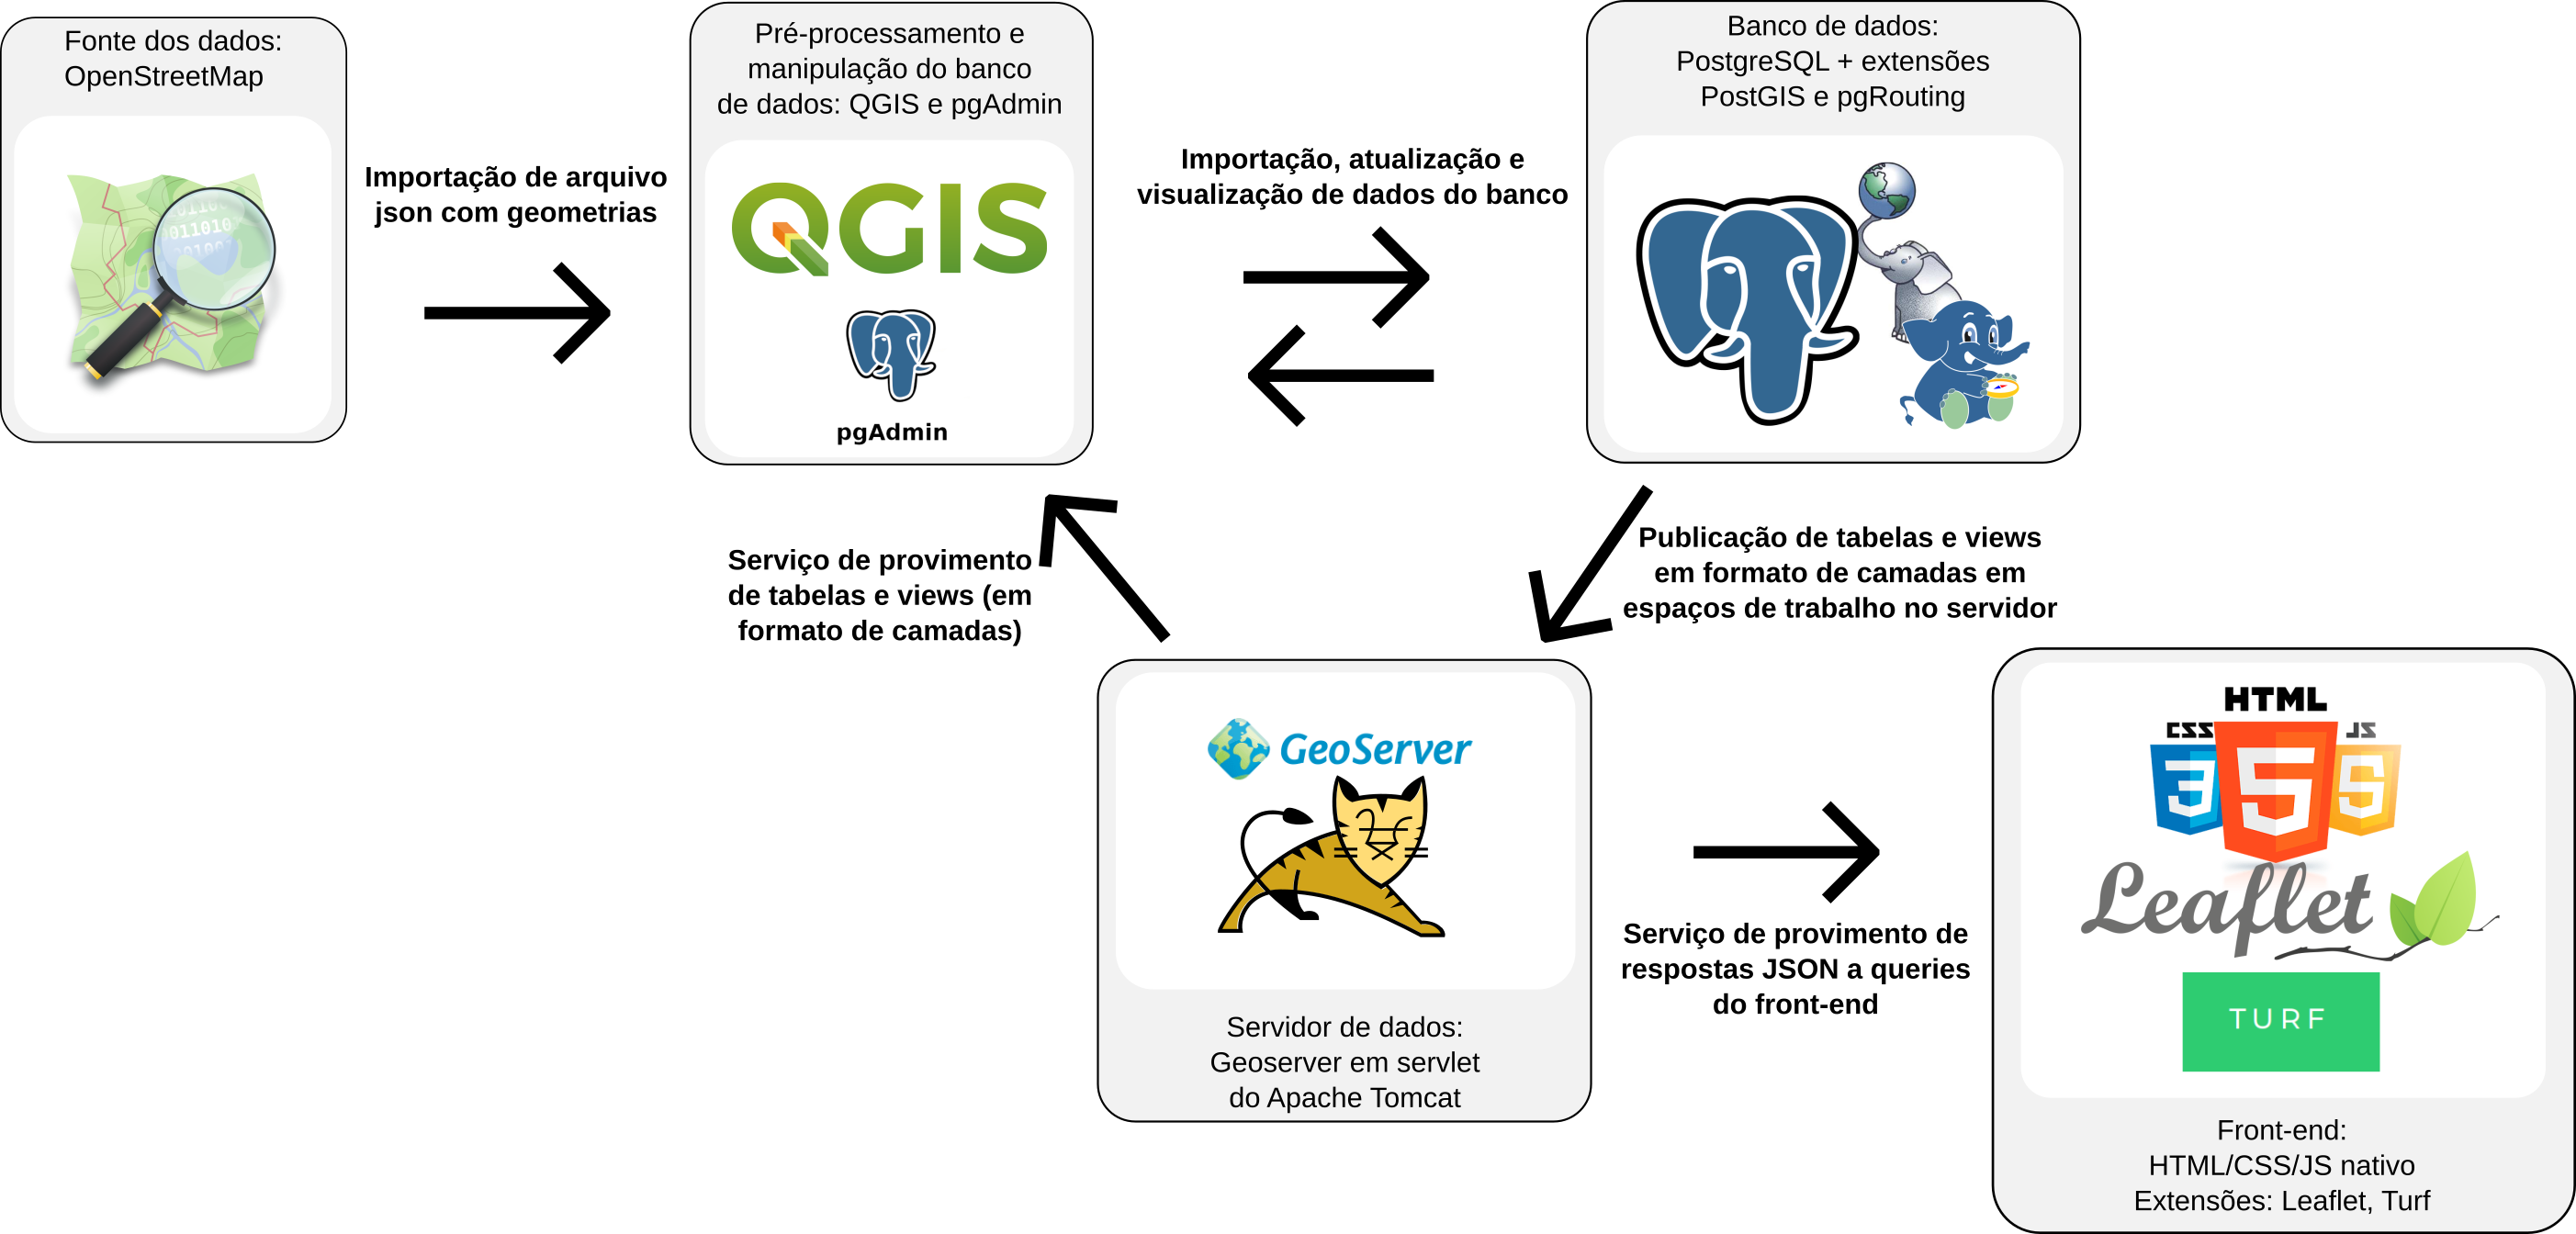
\includegraphics[scale=0.20]{imagens/arq_sistema.png}
    \label{arq_sistema}
    \fonte{Próprio autor.}
\end{figure}

Inicialmente, os dados utilizados para o trabalho são obtidos por consulta ao OpenStreetMap através do site https://overpass-turbo.eu. 
Os dados são então processados no QGIS e importados para o banco de dados PostgreSQL. 
Já no banco de dados, a tabela contendo os segmentos do sistema viário da UFSM são processados para a criação da topologia de rede que permitirá a navegação por meio de algoritmos de busca em grafo.
Também é feita a verificação da rede criada para garantir que ela não contenha erros que possam afetar o cálculo de rotas. 
Após a criação do banco, as camadas de arestas (vias) e vértices (cruzamentos de vias) são publicadas no servidor Geoserver e são criadas as views com consultas para cálculo de rotas e visualização de instalações de acessibilidade em calçadas. 
A aplicação Web é criada logo após a conclusão dos procedimentos necessários no Geoserver.

%\section{Construção da base de dados}
\section{Obtenção de dados estáticos via OpenStreetMap}

A base de dados utilizada pela aplicação é obtida a partir do projeto colaborativo de mapeamento OpenStreetMap. 
Existem diversas formas para extrair dados desta base, desde arquivos pré-processados contendo dados vetoriais de uma região específica do globo (como um país), consultas que englobam todas as geometrias dentro de um polígono regular projetado no mapa, ou arquivos produtos de consultas personalizadas buscando geometrias que atendam a condições específicas, dentre outras formas. 
Neste trabalho, foi utilizada uma consulta personalizada dentro do perímetro do campus Sede da UFSM.

Foi utilizado o serviço oferecido pelo https://overpass-turbo.eu, que requer que as consultas realizadas sobre o OSM sejam feitas numa linguagem de consulta específica, a OverpassQL. 
O código da consulta para a obtenção de todas as ruas que compõem o sistema viário da UFSM disponível no OSM é apresentado na Figura~\ref{codigo:overpass} e o resultado da consulta é mostrado na Figura \ref{screenshot_resultado_overpass}.

\begin{figure}[h!]
    \centering
      \caption{Consulta no Overpass para download de dados}
    \label{codigo:overpass}
    \begin{lstlisting}
[out:json][timeout:25];
{{geocodeArea:UFSM}}->.searchArea;
(
  way["highway"](area.searchArea);
);
out body;
>;
\end{lstlisting}
      \fonte{Próprio autor.}

\end{figure}





%\textcolor{red}{indicar isso de forma mais especifica na figura}
\begin{figure}[ht]
    \caption{Resultado da Consulta ao Overpass Turbo}
    \centering
    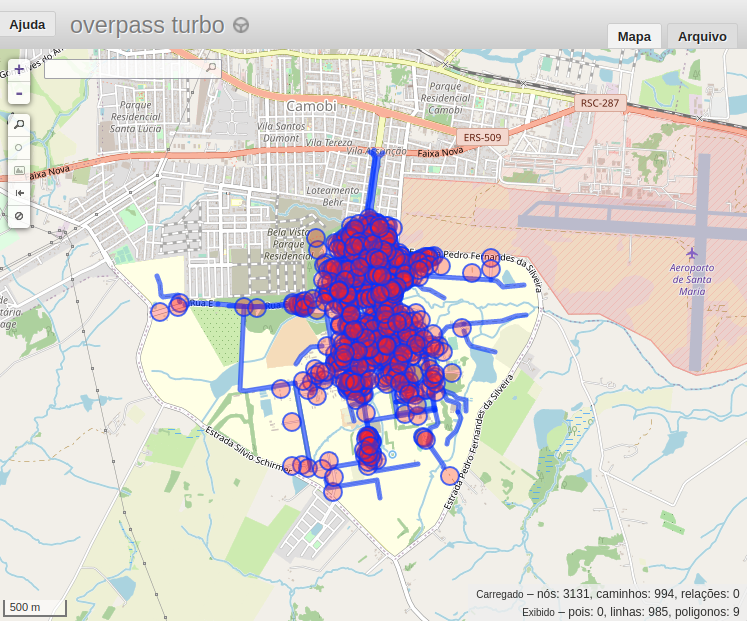
\includegraphics[scale=0.35]{imagens/screenshot_resultado_overpass.png}
    \label{screenshot_resultado_overpass}
    \fonte{Adaptado de https://overpass-turbo.eu.}
\end{figure}

O resultado mostra apenas linhas que contenham o atributo ``highway'' definido, ou seja, todas as linhas que representarem uma via em que seja possível o trafego de pessoas e veículos. 
Aqui, além das calçadas, diversos tipos de via, como ruas de tráfego de automotores e entradas de estacionamento, são recuperados pela consulta porque podem ser úteis no contexto deste trabalho por fornecerem rotas alternativas quando uma rota que seja acessível de ponta a ponta não for encontrada. 
Todas as vias resultantes da consulta estão dentro do polígono que representa os limites do campus Sede da UFSM, exceto a Avenida Roraima que foi recuperada em sua extensão até a RSC-287.


A base de dados do OpenStreetMap é utilizada como fonte de dados para este trabalho porque possui, dentro do campus da UFSM, um alto nível de detalhamento das entidades mapeadas, tanto quantitativa quanto qualitativamente. 
Contudo, outras fontes podem ser consideradas para utilização pela aplicação pelos seguintes motivos:
\begin{itemize}
    \item A Pró-Reitoria de Planejamento da UFSM possui os dados cadastrais oriundos do setor de Geoprocessamento que são de maior confiabilidade.
    \item Apesar da informação cartográfica sobre a UFSM no OSM estar em maior volume do que em outras bases, ainda há informações ausentes sobre o sistema viário.
    \item A base de dados construída para a aplicação pode ser alimentada com outras informações relevantes, como notificações sobre acidentes ou obstáculos em vias.
\end{itemize}
    
    
    
\section{Pré-processamento dos dados}

O pré-processamento de dados é etapa fundamental para a criação de um banco de dados que armazene uma relação ou conjunto de relações suficientemente representativas do sistema viário do campus Sede da UFSM em formato adequado para a etapa de construção de um grafo (ou rede) que suporte a execução dos algoritmos de busca em grafos de maior relevância na literatura.

Neste trabalho, a base é manipulada manualmente, com todos os passos de cada tarefa atrelados a elementos de interface de usuário do QGIS, como menus, botões e caixas de texto. 
Porém, em desenvolvimento futuro, é possível codificar \textit{scripts} Python que fazem uso de bibliotecas de ligação a módulos de processamento de dados vetoriais e matriciais do QGIS para automação dos passos necessários às tarefas de pré-processamento.

As camadas que contém dados geográficos sobre o sistema viário e o limite do perímetro da universidade são importados para o QGIS e o resultado é apresentado na Figura \ref{camadas_importadas_qgis}.

\begin{figure}[h]
    \caption{Resultado da importação de camadas para o QGIS}
    \centering
    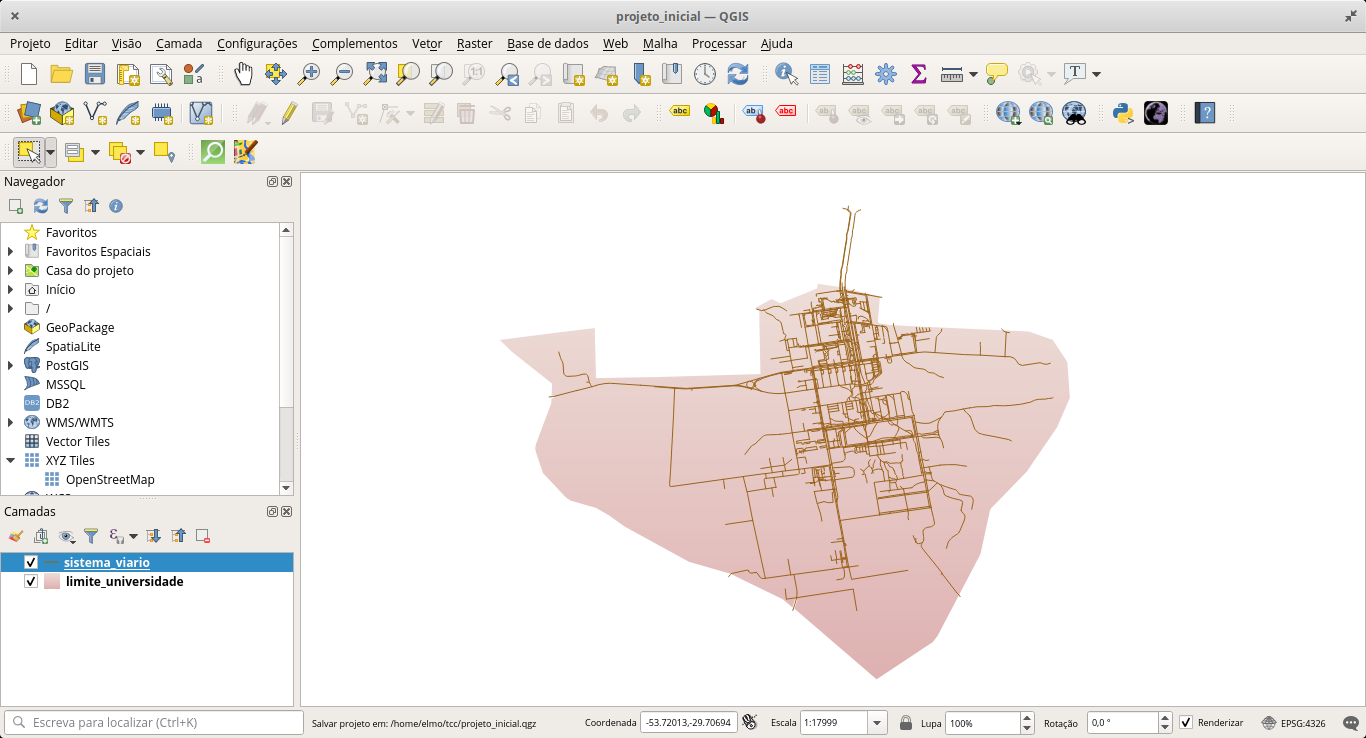
\includegraphics[scale=0.3]{imagens/camadas_importadas_qgis.png}
    \label{camadas_importadas_qgis}
    \fonte{Próprio autor.}
\end{figure}

A primeira etapa do pré-processamento é a reprojeção das camadas do sistema de coordenadas geográficas utilizado pelo OpenStreetMap em coordenadas métricas do SIRGAS 2000, na zona UTM 22 S, para que o processo de medição de comprimento de vias e proximidade entre nós da rede seja simplificado, utilizando unidades métricas em vez de angulares. 
Esta tarefa é executada utilizando os algoritmos de reprojeção de coodernadas do QGIS, acessíveis pelo menu Processar > Caixa de Ferramentas > Vetor Geral > Reprojetar camada. 
A camada de entrada é definida, assim como os SRIDs de origem (camada de entrada) e de destino (camada de saída) são definidos como 4326 e 31982, respectivamente em correspondência aos datums WGS 84 e SIRGAS 2000 UTM Zone 22 S. O diálogo de reprojeção com os campos devidamente preenchidos é mostrado na Figura \ref{dialogo_reprojecao}.

\begin{figure}[h]
    \caption{Diálogo de reprojeção de camadas no QGIS}
    \centering
    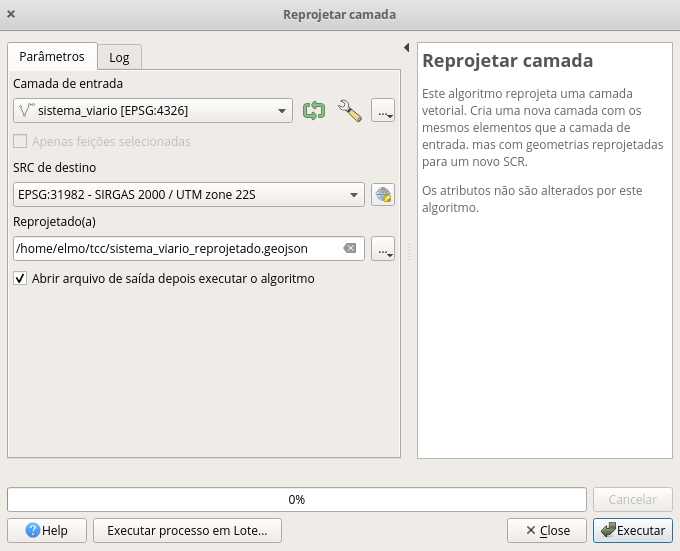
\includegraphics[scale=0.3]{imagens/dialogo_reprojecao.png}
    \label{dialogo_reprojecao}
    \fonte{Próprio autor.}
\end{figure}

A segunda etapa de pré-processamento é o processo de segmentação de linhas conhecido como ``explosão''. 
Este processo divide uma linha em todos os pontos que a constituem, gerando um conjunto de ($np$ - 1) linhas, onde $np$ é o número de pontos na linha.

A terceira tarefa tem a flexibilidade de ser realizada tanto no QGIS quanto por meio de cliente do Postgres, a exemplo do pgAdmin. 
Nesta tarefa, ocorre a limpeza de colunas (ou atributos) relacionados às geometrias. 
Algumas colunas não são úteis para as aplicações que executam consultas à base de dados, outras estão com dados ausentes ou incompletos, necessitando de tratamento.
O tratamento pode ser manual ou automatizado no QGIS por meio de scripts em Python ou no Postgres por meio de scripts SQL. 



\section{Criação do banco de dados}

\subsection{Importação de dados}
A importação dos dados para o banco de dados é feita por meio de um utilitário shp2-pgsql-gui que acompanha a instalação padrão do PostGIS. 
A importação poderia ser realizada por meio deste mesmo utilitário em sua versão para linha de comandos, ou pelo utilitário ogr2ogr que faz a conversão e importação entre diversas fontes e diversos destinos de formatos geográficos disponíveis.

Há outra ferramenta, específica para dados do OpenStreetMap, que além de realizar a importação, também faz verificações topológicas e constrói a rede viária, tornando o grafo resultante pronto para utilização.
Entretanto, como este trabalho tem por objetivo propôr uma arquitetura que seja composta por módulos que sejam inteligíveis a profissionais de outras áreas e que proporcione a flexibilidade e multiplicidade de fontes de dados que alimentarão o banco, de todas as opções citadas, o utilitário com interface gráfica é o mais adequado. 
A Figura \ref{shp2pgsql} apresenta o diálogo de importação do utilitário.


\begin{figure}[h!]
    \caption{Janela de diálogo do shp2sql-gui}
    \centering
    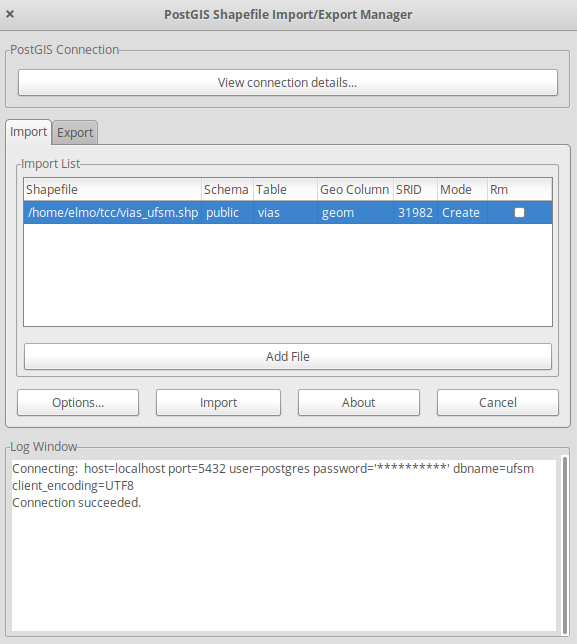
\includegraphics[scale=0.3]{imagens/shp2pgsql.png}
    \fonte{Próprio autor.}
    \label{shp2pgsql}
\end{figure}

\subsection{Verificação e criação da topologia de rede}

Após a importação dos dados, a etapa de verificação de geometrias e criação da topologia da rede é necessária. 
A extensão {\tt pgRouting} oferece funções bem documentadas que realizam a importante etapa de verificação de topologia para que a rede criada seja navegável e garanta a correta ligação entre nós (vértices) e vias (arestas).
A função {\tt pgr\_createtopology()} cria a topologia de rede a partir da coluna  {\tt geom}  que armazena geometrias na tabela {\tt vias}, importada na etapa anterior. 
A assinatura da função é mostrada na Figura~\ref{codigo:create_topology}.

\begin{figure}[h!]
    \centering
     \caption{Assinatura da função {\tt pgr\_createTopology()}}
    \label{codigo:create_topology}
    \begin{lstlisting}
varchar pgr_createTopology(text edge_table, 
       double precision tolerance,
       text the_geom := `the_geom',
       text id := `id',
       text source := `source',
       text target := `target',
       text rows_where := `true',
       boolean clean := false)
\end{lstlisting}
   \fonte{Próprio autor.}
\end{figure}


O parâmetro {\tt edge\_table} deve receber o nome da tabela onde estão armazenadas as geometrias do tipo linha representando o sistema viário. 
Logo, deve ser substituído pelo nome da tabela importada: {\tt vias}.

O parâmetro {\tt tolerance} deve receber um valor real que indique qual a distância máxima entre as extremidades de duas linhas diferentes para que elas sejam consideradas conectadas. 
Este valor deve ser informado considerando o sistema de referência da tabela {\tt vias}, que é métrico. Aqui o valor definido foi 0.01, correspondendo a 1 centésimo de metro, ou 1 centímetro.

O parâmetro {\tt the\_geom} deve ser substituído pelo nome da coluna da tabela {\tt vias} que armazena a representação geométrica em WTK (Well Known Text) de cada registro (ou segmento), aqui chamada de {\tt geom}.

O parâmetro {\tt id} deve ser substituído pela nome da chave primária da tabela {\tt vias}, com o mesmo nome: {\tt id}.

O parâmetros {\tt source} e {\tt target} serão preenchidos com os identificadores de vértices de origem e destino de cada aresta. 
Os vértices serão criados como geometria de ponto e alocados em uma nova tabela, com o nome {\tt vias\_vertices\_pgr}, após a execução da consulta. Caso estas colunas ainda não existam na tabela {\tt vias}, é preciso criá-las antes de executar a consulta.

Os parâmetros {\tt rows\_where} e {\tt clean} servem como filtro de geometrias e indicação de criação de topologia que sobrescreva totalmente a criada em consultas anteriores. Eles não são relevantes para a consulta atual, então serão omitidos e assumirão seus valores padrão.

Com as substituições descritas, a consulta a ser executada no pgAdmin (ou qualquer outro cliente do PostgreSQL) é a mostrada na Figura~\ref{codigo:create_topology_final}.

\begin{figure}[h!]
    \centering
    \begin{lstlisting}[]
    select pgr_createTopology(`vias', 0.01, `geom', `id', `source', `target');
\end{lstlisting}
    \caption{Função {\tt pgr\_createTopology()} após substituição de argumentos}
    \label{codigo:create_topology_final}
      \fonte{Próprio autor.}
\end{figure}



A consulta retorna {\tt OK} após ser executada com sucesso. É então criada uma nova tabela ({\tt vias\_vertices\_pgr}) contendo os vértices calculados a partir das intersecções entre uma ou mais arestas da rede na tabela {\tt vias}. 
A nova tabela contém as seguintes colunas:


\begin{itemize}
    \item {\tt id}: chave primária do vértice
    \item {\tt cnt}: quantidade de arestas na tabela {\tt vias} que fazem referência aos vértices seja na coluna {\tt target} ou na coluna {\tt source}
    \item {\tt chk}: indicação de possível problema no vértice
    \item {\tt ein}: quantidade de arestas que referenciam este vértice como sendo de destino
    \item {\tt eout}: quantidade de arestas que referenciam este vértice como sendo de origem
    \item {\tt the\_geom}: representação geométrica do vértice
\end{itemize}

A próxima etapa na criação da rede é a análise do grafo resultante para a busca de possíveis problemas como vias sobrepostas sem vértices registrados em tais intersecções, circuitos isolados sem conexão com a rede principal ou "becos sem saída". A função {\tt pgr\_analyzeGraph()} executa esta análise e a assinatura dela é mostrada na Figura~\ref{codigo:analyzeGraph}.

\begin{figure}[h!]
    \centering
      \caption{Assinatura da função {\tt pgr\_analyzeGraph()}}
    \label{codigo:analyzeGraph}
    \begin{lstlisting}[]
varchar pgr_analyzeGraph(text edge_table,
                    double precision tolerance,
                    text the_geom := `the_geom',
                    text id := `id',
                    text source := `source',
                    text target := `target',
                    text rows_where := `true')    
\end{lstlisting}
    \fonte{Próprio autor.}
\end{figure}




Os parâmetros da função {\tt pgr\_analyzeGraph()} são exatamente os mesmos da função {\tt pgr\_createTopology()} utilizada anteriormente. 
Com as devidas substituições, a consulta a ser executada é mostrada na Figura~\ref{codigo:analyzeGraph_final-1}

\begin{figure}[h!]
    \centering
    \caption{Consulta com {\tt pgr\_analyzeGraph()} após substituição de argumentos}
    \label{codigo:analyzeGraph_final-1}
    \begin{lstlisting}[]
select pgr_analyzeGraph(`vias', 0.01, `geom', `id', `source', `target');
\end{lstlisting}
 \fonte{Próprio autor.}
\end{figure}


É importante atentar à obrigatoriedade de topologia já existente antes de executar a consulta, com a tabela de arestas {\tt vias} e a tabela de vértices {\tt vias\_vertices\_pgr} associada. 
Caso contrário, a função retornará {\tt FAIL}. 
A consulta apresentada na Figura~\ref{codigo:analyzeGraph_final-1} é executada, retorna {\tt OK} e também mostra um relatório contendo os resultados encontrados, vide Figura~\ref{relatorio}. 
A parte do relatório que importa ao trabalho é mostrado na transcrição abaixo.


\begin{figure}
    \centering
     \caption{Relatório com o resultado da consulta apresentada na Figura~\ref{codigo:analyzeGraph_final-1}}
    \label{relatorio}
    \begin{verbatim}
NOTICE:              ANALYSIS RESULTS FOR SELECTED EDGES:
NOTICE:                    Isolated segments: 10
NOTICE:                            Dead ends: 302
NOTICE:  Potential gaps found near dead ends: 0
NOTICE:               Intersections detected: 9
NOTICE:                      Ring geometries: 0  
\end{verbatim}
    \fonte{Próprio autor.}
\end{figure}





Observando o relatório, é possível verificar que 10 {\tt Isolated segments} (segmentos isolados) foram encontrados. 
Estes segmentos representam pequenos caminhos em regiões mais afastadas do campus e que não afetam o roteamento na rede principal. 
Caso o número de segmentos isolados fosse uma porcentagem alta do total de segmentos, seria necessária uma verificação aprofundada em busca de problemas no pré-processamento ou criação da topologia.
A tabela {\tt vias} contém mais de 3500 segmentos e os segmentos isolados são apenas 10.

Quanto aos {\tt dead ends}, são apenas segmentos em que um de seus vértices não possuem arestas de saída, apenas de entrada. 
Não são erros de topologia, pois representam a realidade de ruas, calçadas e quaisquer outras categorias de vias que tem sua extensão encerrada em algum ponto (vértice) da rede.

Não foram encontradas {\tt ring geometries}, traduzidos livremente para ``geometrias de anel", que são circuitos fechados com três ou mais segmentos conectados em um ciclo e que estão isolados da rede principal. 

Também não foram encontradas lacunas potencialmente inseridas por erro de aderência entre dois segmentos que deveriam estar conectados, de acordo com a distância máxima entre extremidades, definida como 0.01 ou 1 centímetro.

As intersecções encontradas foram 9 e por conhecimento empírico do sistema viário do campus Sede da UFSM, é possível identificar o local onde elas acontecem: nas intersecções em diferentes níveis entre a ponte da Avenida Roraima e as vias de circulação de veículos, pedestres e bicicletas que passam sob esta ponte. O local onde as intersecções ocorrem podem ser observados na Figura \ref{fig:cinco}.

A função {\tt pgr\_nodeNetwork()} pode ser utilizada para corrigir erros de topologia em uma rede que não está "nodada", com todas as intersecções entre linhas devidamente registradas. Porém, como as intersecções sem registro de vértice comum são inerentes à rede no caso do campus Sede da UFSM, não há necessidade da execução deste passo.
Outro fator preponderante para a não-utilização da função é a complexidade adicional que ela adiciona às consultas de pesquisa de rotas, visto que o sistema viário é representado por duas tabelas ao invés de uma, a primeira com o sistema viário original e a segunda com o sistema viário ``nodado", referenciando pelo campo {\tt old\_id} o segmento do qual teve origem.




\begin{figure}[ht]
\caption{Fotografias e representações vetoriais da ponte da Avenida Roraima}
\center
\subfigure[Calçada da ponte na Avenida Roraima.]{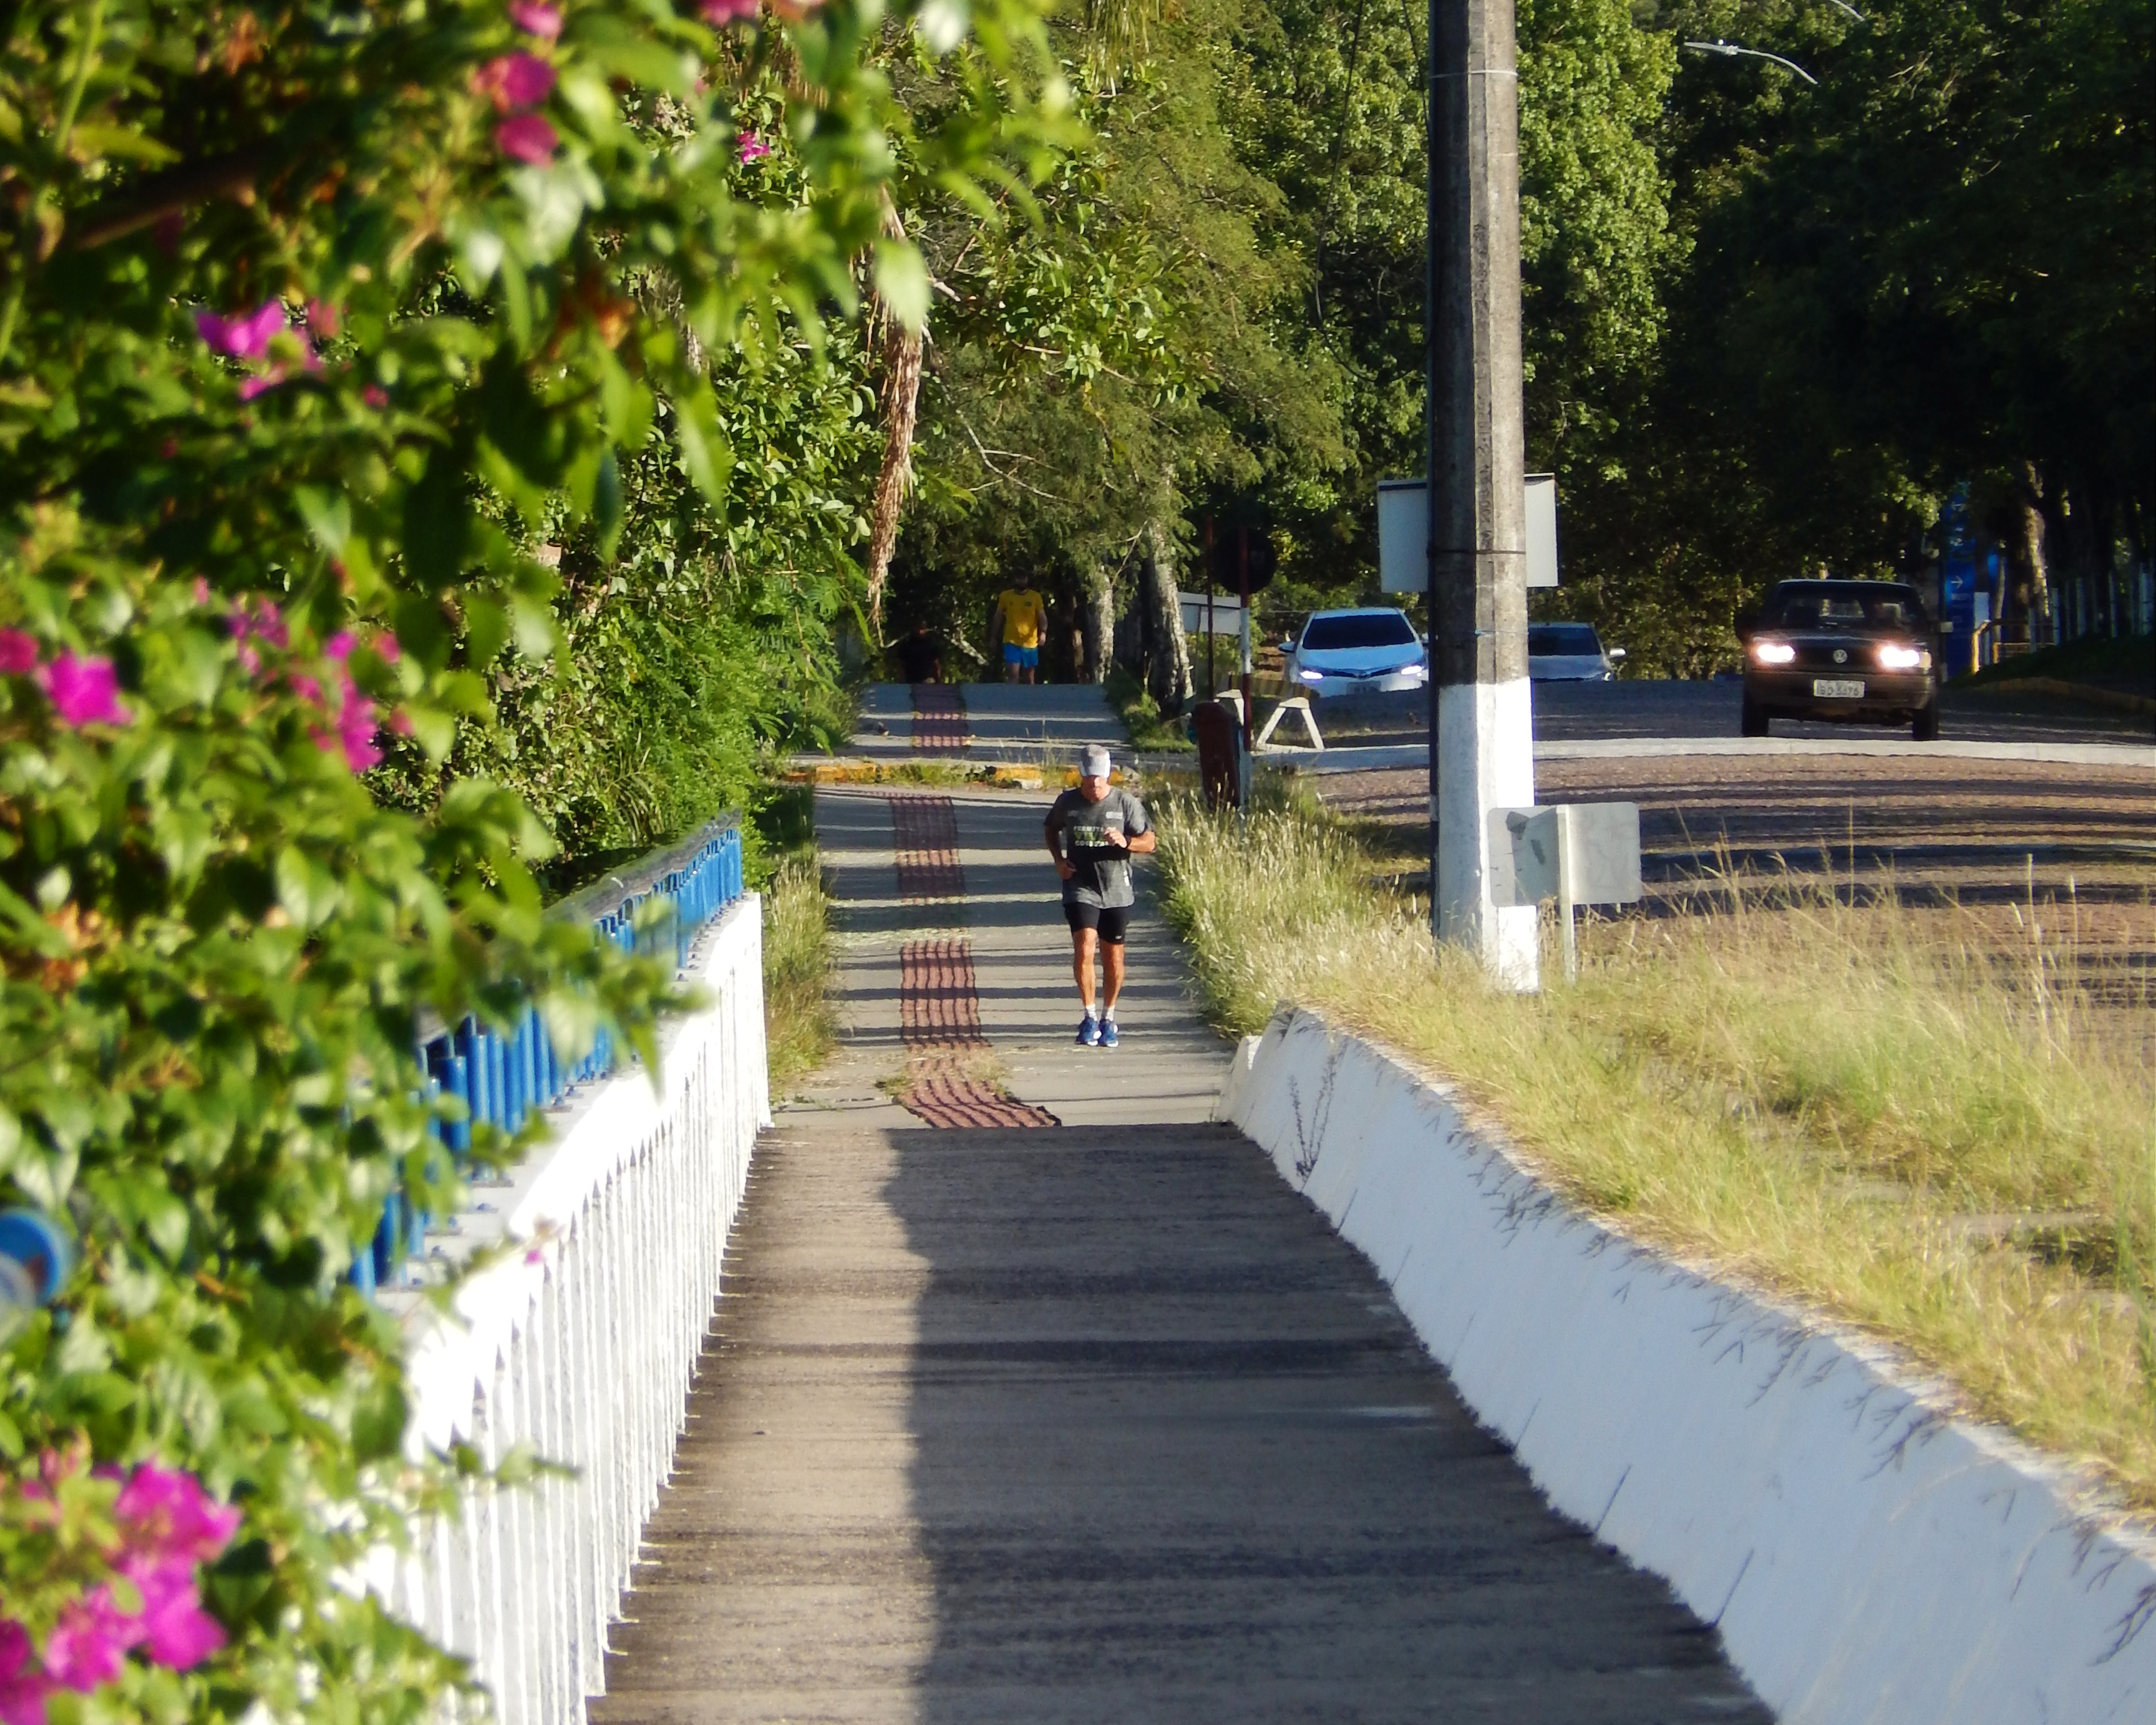
\includegraphics[width=0.45\textwidth]{imagens/ponte_foto_1.JPG}}
\qquad
\subfigure[Pista multiuso da UFSM.]{ 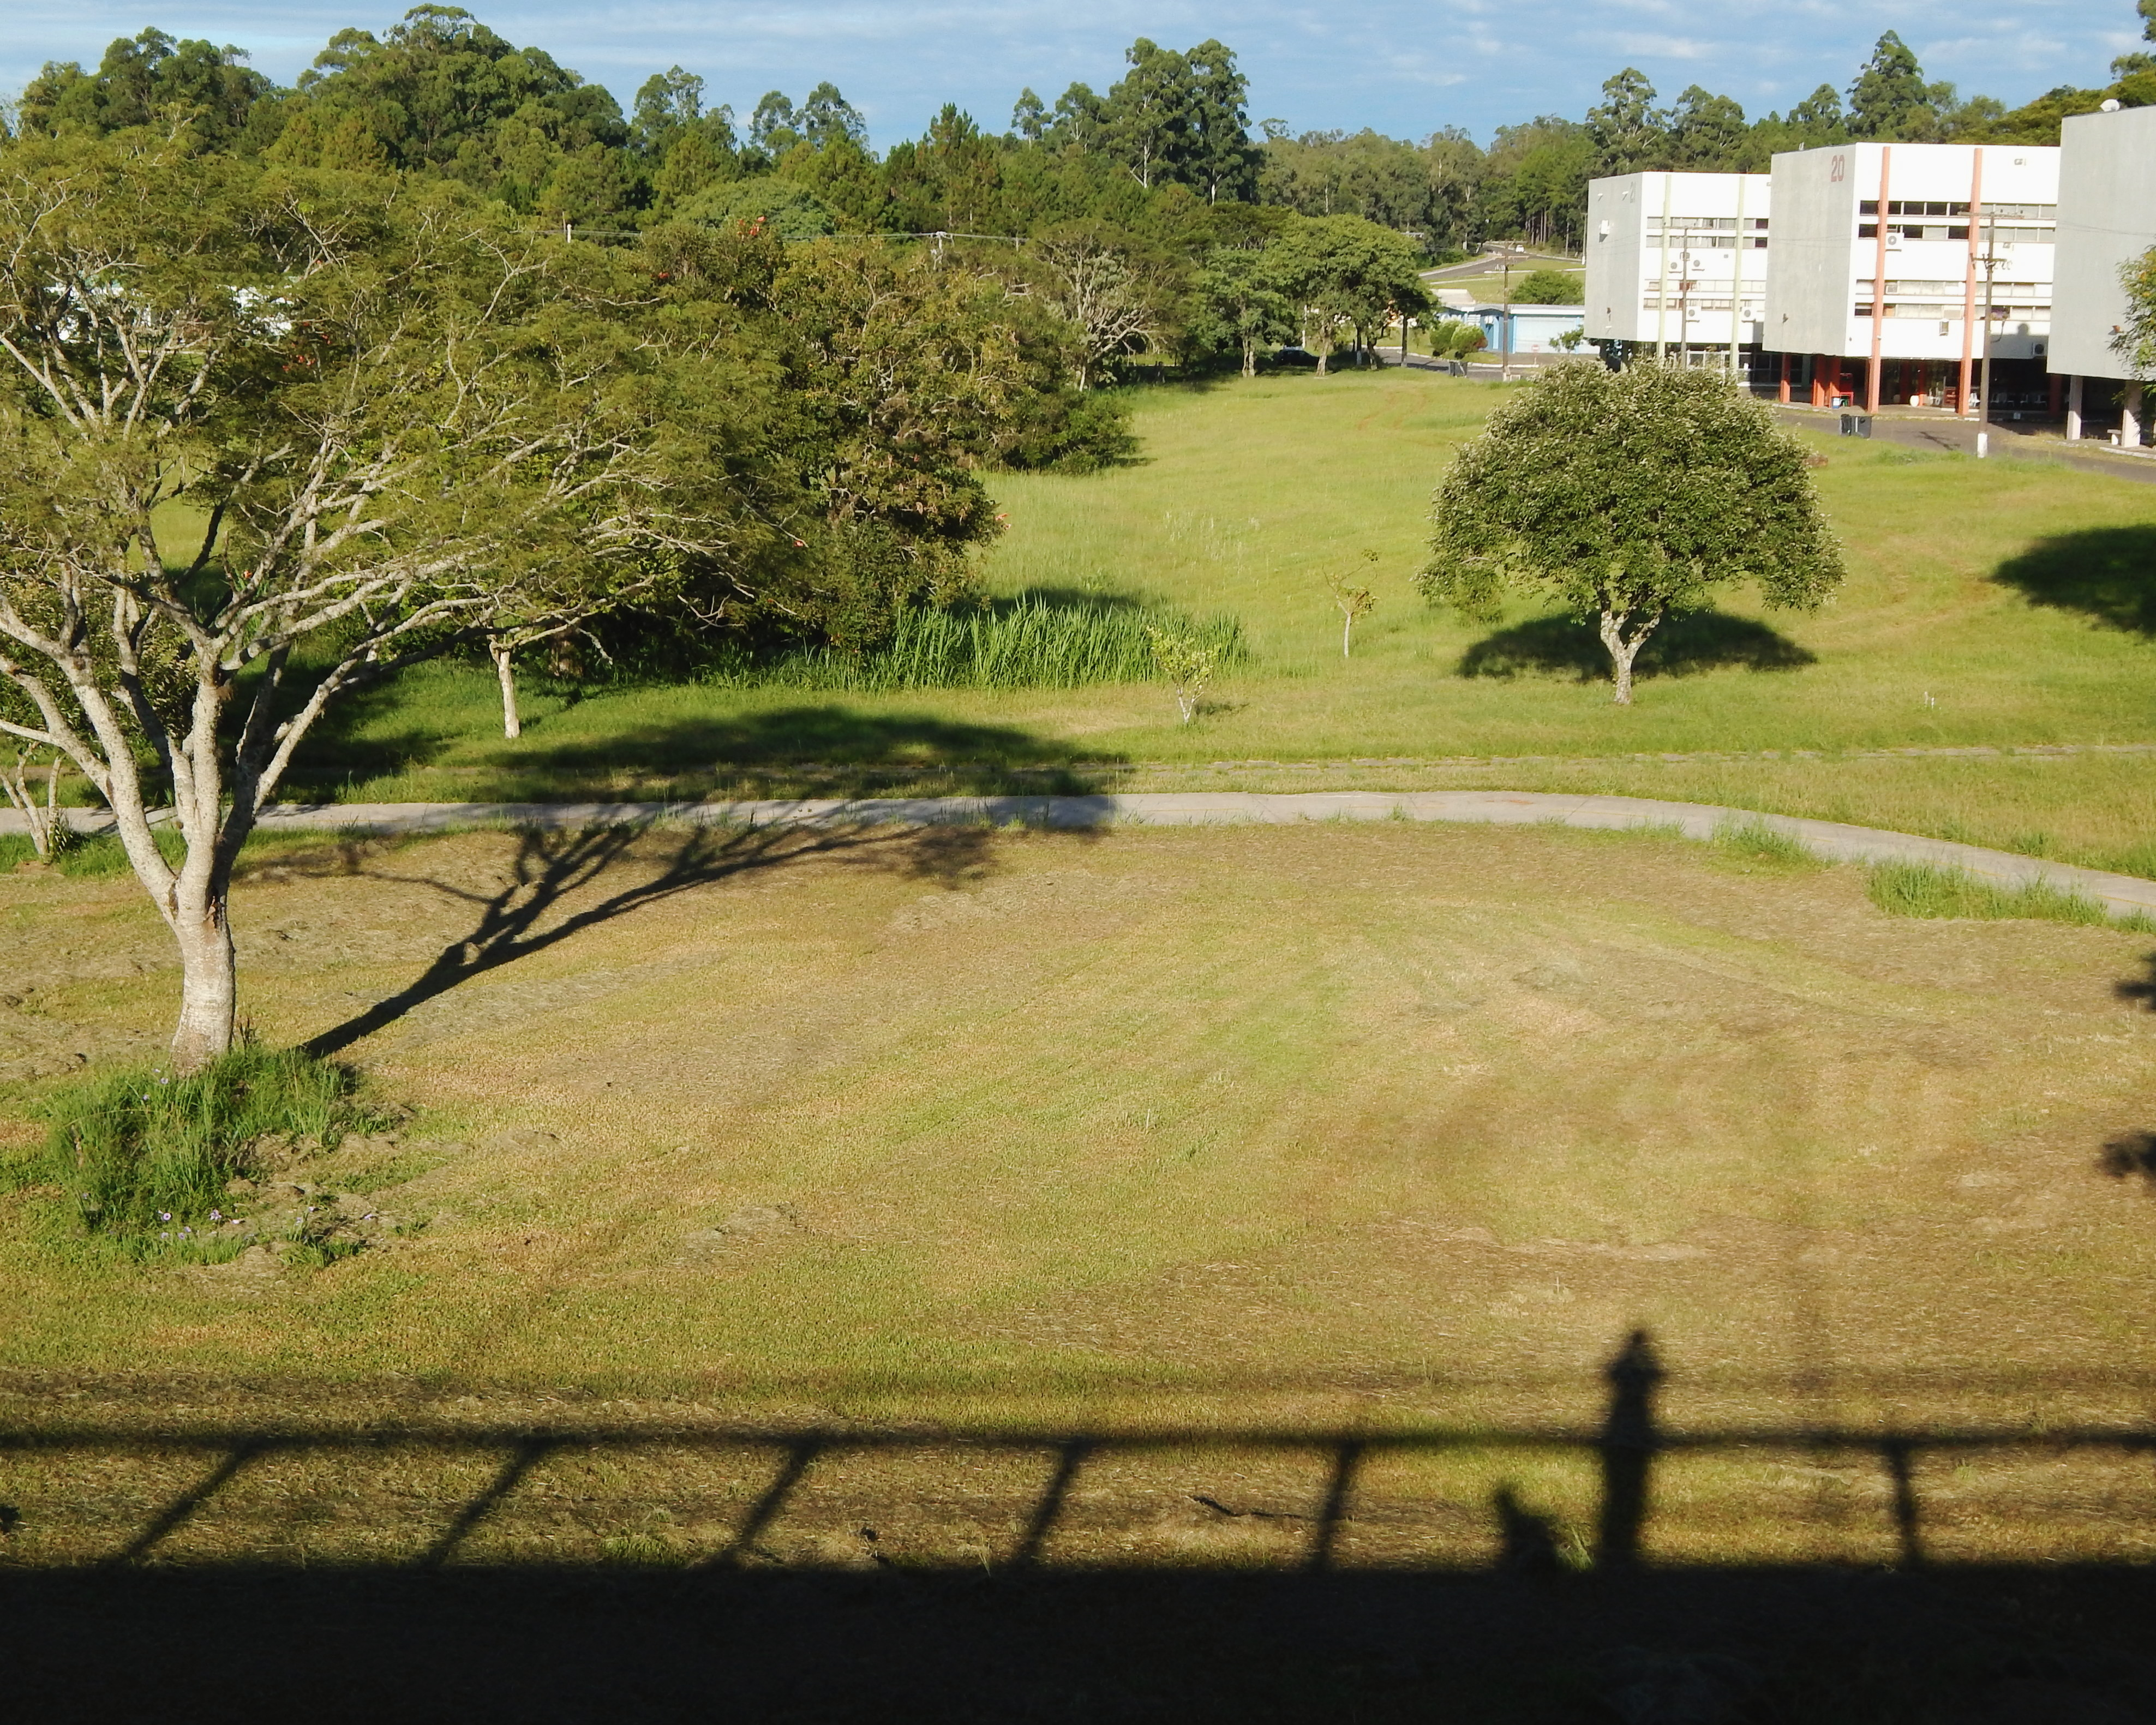
\includegraphics[width=0.45\textwidth]{imagens/ponte_foto_2.JPG}}
\subfigure[Ponte da Avenida Roraima no OSM.]{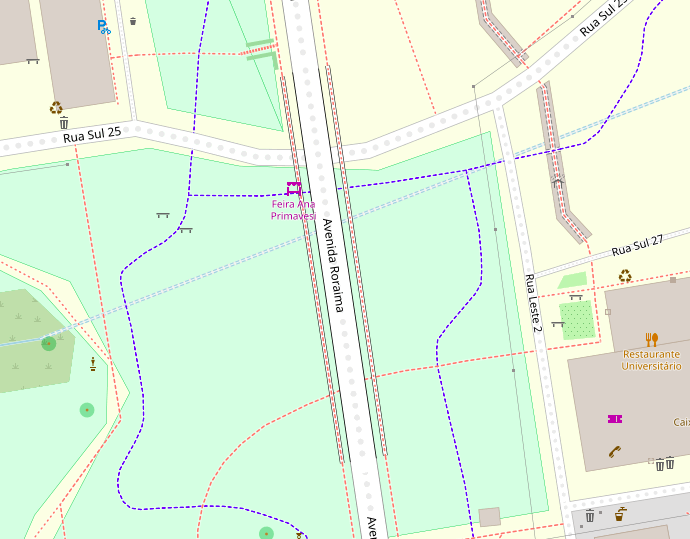
\includegraphics[width=0.45\textwidth]{imagens/ponte_osm.png}}
\qquad
\subfigure[Ponte da Avenida Roraima no QGIS.]{ 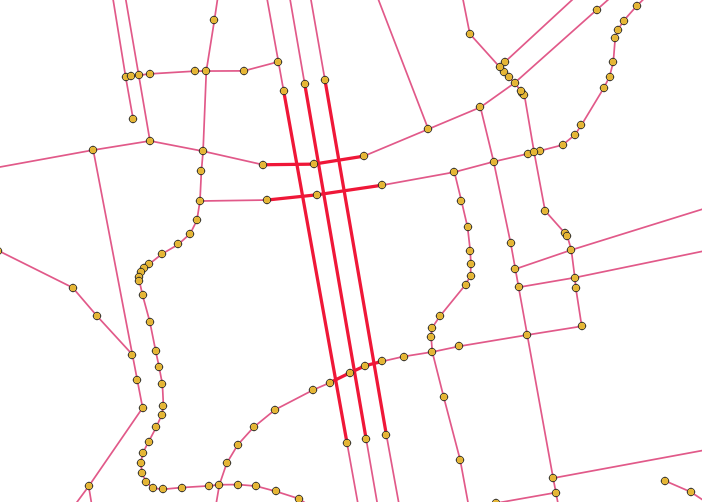
\includegraphics[width=0.45\textwidth]{imagens/ponte_qgis.png}}




\label{fig:cinco}
\fonte{(a) e (b) acervo pessoal do autor, (c) adaptado de OpenStreetMap e (d) próprio autor.}
\end{figure}





\subsection{Adição de colunas de reprojeção e custo}


Após a criação da topologia de rede e verificação de possíveis problemas, é necessária a criação de  colunas adicionais que serão úteis ou obrigatórias para consultas de pesquisa em grafo e para visualização de geometrias em mapas na Web.
Por exemplo, para tornar possível a execução do Algoritmo de Dijkstra sobre o grafo (ou rede), a coluna {\tt custo} deve ser criada, inicialmente calculada a partir do comprimento em metros de cada segmento.  
O custo de cada segmento também foi alterado durante o trabalho para efeito de testes, onde as vias de maior circulação de veículos receberam um fator multiplicador que aumentava seu custo e as calçadas e pista multiuso receberam um fator multiplicador que diminuía seu custo.

Em trabalhos futuros, é importante mencionar que o cálculo apresentado na Figura~\ref{codigo:coluna_custo} deve  considerar outros atributos, como a declividade do terreno onde a via se encontra. 
Este atributo específico pode ser extraído do cruzamento entre a base vetorial do sistema viário da universidade e curvas de nível também em formato vetorial obtidas a partir de levantamentos topográficos realizados pela UFSM.

\begin{figure}[h!]
    \centering
        \caption{Consulta para criação de coluna de custo de aresta}
    \label{codigo:coluna_custo}
\begin{lstlisting}[]
ALTER TABLE vias
ADD custo real;

UPDATE TABLE vias
SET custo = ST_Length(geom)
\end{lstlisting}
   \fonte{Próprio autor.}
\end{figure}


A função  {\tt ST\_Length()} calcula o comprimento da geometria utilizando como parâmetro a coluna {\tt geom} de cada registro. 
É necessário que o sistema de referência de coordenadas utilizado seja métrico, e como o datum utilizado para os dados foi o SIRGAS 2000 / UTM Zone 22 S, não há necessidade de reprojeção antes do cálculo.

A visualização de mapas na Web e em aplicativos de dispositivos móveis utilizam um datum diferente do utilizado nas tabelas do banco de dados criado. 
O sistema de referência de coordenadas não é projetado na superfície terrestre, utilizando medidas angulares de latitude e longitude. O datum mais comum para visualização de mapas na Web é o WGS 84. 
Por este motivo, nas duas tabelas, de arestas e vértices, foram criadas colunas que armazenam suas geometrias segundo este sistema, tornando mais simples a recuperação e visualização de dados espaciais em páginas Web e aplicativos. 
A consulta para a criação e preenchimento desta coluna é mostrada na Figura~\ref{codigo:coluna_reprojecao}.

\begin{figure}[h!]
\center
      \caption{Consulta para criação de coluna de reprojeção}
    \label{codigo:coluna_reprojecao}
    \begin{lstlisting}
SELECT AddGeometryColumn (`public',`vias', `geom_4326', 4326, `LINESTRING', 2);
UPDATE vias
SET geom_4326 = ST_Transform(geom,4326)
\end{lstlisting}
   \fonte{Próprio autor.} 
\end{figure}


A função {\tt AddGeomtryColumn()} está presente na instalação padrão da extensão PostGIS e recebe como parâmetros o nome do esquema e da tabela que serão alteradas e o nome da coluna que será adicionada: {\tt geom\_4326}. 
Também recebe os parâmetros como o sistema de referência de coordenadas da coluna, o tipo de geometria a ser armazenada e em quantas dimensões ela está representada. 
O SRID desta coluna é {\tt 4326} (código EPSG para WGS 84), o tipo de geometria é LINESTRING e como não há medição de altitude para as geometrias (eixo Z), o número de dimensões é 2.

A função {\tt ST\_Transform} também é da instalação padrão do PostGIS. 
Ela faz a reprojeção de um sistema de coordenadas de referência para outro. 
Aqui ela faz a reprojeção do datum SIRGAS 2000 / UTM Zone 22 S para o WGS 84.

O procedimento para a tabela de vértices é semelhante, apenas fazendo a substituição do nome da tabela para {\tt vias\_vertices\_pgr} e alterando o tipo da geometria para POINT.

Todas as etapas aqui descritas podem ser automatizadas por meio de {\tt scripts} e {\tt triggers} para tornar a rede viária pronta para utilização logo após a importação.

\section{Conexão com o QGIS}


A conexão com o QGIS serve como auxílio para testes e visualização de resultados plotados em ambiente cartográfico, além de fornecer um ambiente mais amigável para profissionais responsáveis por mapeamento de instalações físicas no campus Sede da UFSM. 
A instalação padrão do QGIS fornece ferramentas de conexão com o banco de dados PostgreSQL e também uma janela de consulta SQL. 
A conexão com o banco de dados é feita através da janela de diálogo na Figura \ref{dialogo_conexao_banco_qgis} e as tabelas do banco importadas como camadas para o QGIS podem ser vistas na Figura~\ref{camadas_banco_qgis}. 

\begin{figure}[h!]
    \caption{Diálogo de conexão do banco de dados com o QGIS}
    \centering
    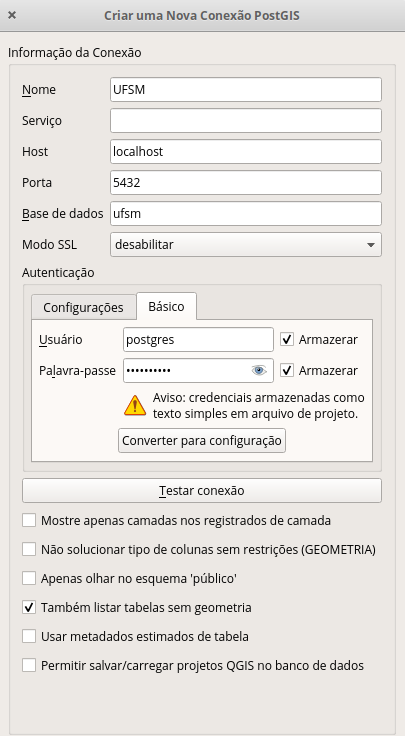
\includegraphics[scale=0.3]{imagens/dialogo_conexao_banco_qgis.png}
    \label{dialogo_conexao_banco_qgis}
    \fonte{Próprio autor.}
\end{figure}

\begin{figure}[h!]
    \caption{Tabelas do banco de dados importadas como camadas no QGIS}
    \centering
    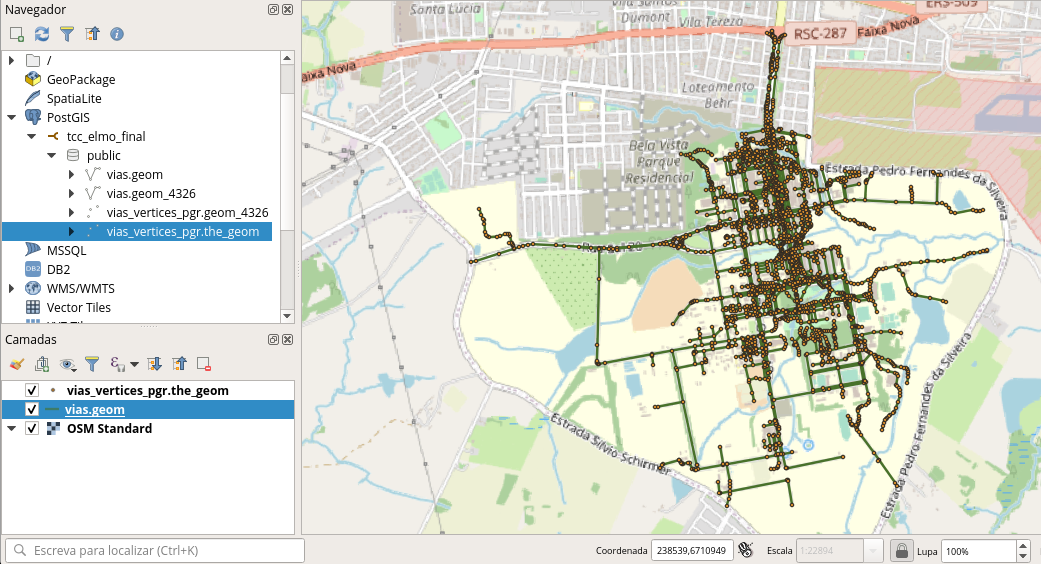
\includegraphics[scale=0.4]{imagens/camadas_banco_qgis.png}
    \fonte{Próprio autor.}
    \label{camadas_banco_qgis}
\end{figure}

\section{Configuração do Servidor}

O GeoServer foi instalado em um servlet do servidor Apache Tomcat, versão 9. A instalação é simples, requerindo apenas a cópia do arquivo .war de deploy disponível na página oficial do GeoServer para dentro da pasta de Web Apps do Tomcat. 
Dispõe de uma interface Web onde é possível acessar configurações globais do servidor e configurações de cada um dos espaços de trabalho com seus respectivos armazéns e camadas de dados.

\subsection{Criação de espaços de trabalho e armazéns de dados}

A configuração tem início com a criação de um espaço de trabalho para alocação dos armazéns e camadas de dados que serão publicados e se tornarão acessíveis por clientes. 
É interessante o isolamento de diferentes setores de instituições em diferentes espaços de trabalho para uma melhor organização de permissões de acesso a dados.

O espaço de trabalho aqui criado tem o nome de {\tt ufsm} e a lista de espaços de trabalho é atualizada, contando agora com o espaço recém-criado, além daqueles que estão presentes na instalação padrão do GeoServer, como mostrado na Figura~\ref{fig:workspace}.
O diálogo de criação do espaço de trabalho é simples, sendo necessário o preenchimento do campo que dá nome ao espaço.

\begin{figure}[h!]
\caption{Listagem de Espaços de Trabalho do GeoServer}
    \centering
    \includegraphics[scale=0.4]{imagens/workspaces_Geoserver.png}
    \fonte{Próprio autor.}
    \label{fig:workspace}
\end{figure}

Após a criação do espaço de trabalho, é feita a criação do armazém de dados que pode ter como fonte de dados arquivos de dados geográficos vetoriais ou matriciais, um diretório contendo vários destes arquivos ou uma banco de dados geográfico, dentre outros. 
Aqui a opção "PostGIS Database'' será selecionada, pois condiz com o banco de dados construído na etapa anterior.

As informações necessárias na janela de diálogo são as de conexão com o banco de dados, como nome do host, nome da base, nome do usuário e senha.
Também é possível definir número máximo de conexões simultâneas, tempo limite de resposta, dentre outras configurações. A listagem de ``stores'' ou  ``armazéns de dados'' disponíveis é mostrada na Figura \ref{stores_geoserver}.

\begin{figure}[ht]
    \caption{Listagem de Armazéns de Dados do GeoServer}
    \centering
    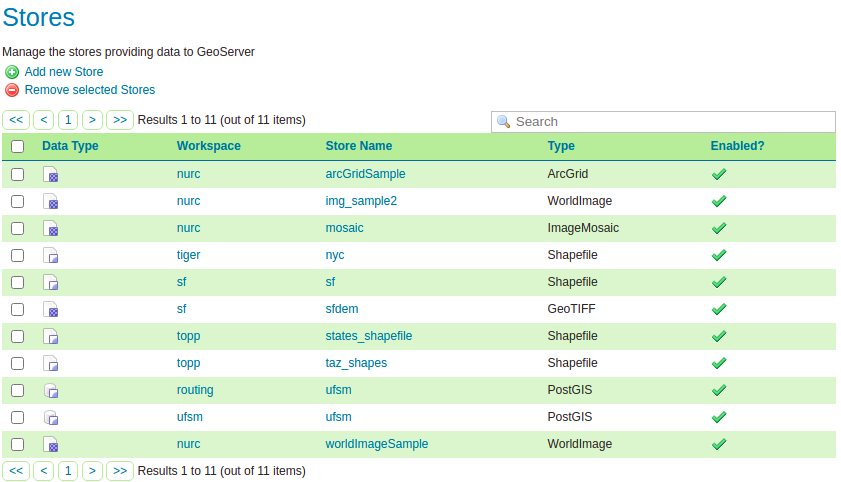
\includegraphics[scale=0.4]{imagens/stores_geoserver.png}
    \fonte{Próprio autor.}
    \label{stores_geoserver}
\end{figure}

\subsection{Criação de views}

Em sequência à criação de armazéns de dados, a etapa principal da configuração do servidor é a disponibilização de camadas vetoriais do banco por meio da função "Publicar''. 
Além de publicação das tabelas do banco de dados, é necessário criar views resultantes das consultas essenciais à aplicação proposta por este trabalho. 
Três views serão criadas e disponibilizadas para clientes, os quais podem ser aplicações Web, aplicações nativas do sistema operacional Android, entre outros. 

\begin{itemize}
    \item {\tt busca\_vertice\_proximo:} busca no banco de dados o vértice geometricamente mais próximo do marcador de mapa informado pelo usuário ou da sua localização obtida por GNSS
    \item {\tt calcula\_rota:} executa o cálculo de rota entre os dois vértices atuais recebidos como entrada a partir da(s) resposta(s) da view {\tt busca\_vertice\_proximo}
    \item {\tt busca\_todas\_rampas:} retorna todas as geometrias do tipo ponto no banco de dados que representam rampas de acesso a calçadas
\end{itemize}    
    A view {\tt busca\_vertice\_proximo} recebe dois parâmetros, {\tt x} e {\tt y}, que representam as coordenadas geográficas do ponto associado ao marcador de mapa ou posição GNSS do usuário. A função {\tt ST\_MakePoint()} cria uma geometria temporária do tipo ponto e a função {\tt ST\_SetSRID()} associada a ela um SRID, no caso, o código 4326 correspondente ao datum WGS 84. Na subconsulta em que está inserida, esta geometria é um dos operandos do operador de distância entre geometrias $< - >$. O outro operando é representado por cada um dos vértices da tabela. O resultado é então ordenado do vértice com a menor distância para o vértice com mair distância até a geometria criada. O ponto de menor distância é então selecionado. A condição logo após a subconsulta é inserida para garantir que este ponto mais próximo esteja conectado à rede, verificando se seu identificador está associado ao ponto de partida ou chegada de uma aresta. São então retornados pela consulta o atributo {\tt id} do vértice mais próximo e sua geometria.
O código da view é mostrado é mostrado na Figura~\ref{codigo:view_vertice}.
   
   
\begin{figure}[h!]
    \centering
      \caption{Código da view \tt{busca\_vertice\_proximo}}
    \label{codigo:view_vertice}
\begin{lstlisting}[]
SELECT v.id, v.geom_4326
FROM vias_vertices_pgr AS v, vias AS a
WHERE v.id = (SELECT id
            FROM vias_vertices_pgr
            ORDER BY geom_4326 <->
            ST_SetSRID(ST_MakePoint(%x%, %y%), 4326) LIMIT 1)
            AND (v.source = a.id OR v.target = a.id)
GROUP BY v.id, v.geom_4326
\end{lstlisting}
  
       \fonte{Próprio autor.}
\end{figure} 


A view {\tt calcula\_rota} recebe três parâmetros: os pontos de origem e destino, representados por {\tt source} e {\tt target}, respectivamente e um filtro, representado por {\tt filtro} para a escolha de que tipo de vias serão utilizadas para o cálculo da rota. 
A função {\tt pgr\_dijkstra()} da instalação padrão do pgRouting faz o cálculo do caminho de menor distância entre dois vértices utilizando o algoritmo de Dijkstra, amplamente difundido na literatura. 
Recebe como argumento o resultado de uma subconsulta, o identificador do vértice de origem, o identificador do vértice de destino e um parâmetro booleano que determina se o grafo é direcionado ou não. 
A subconsulta exige que sejam especificados: o identificador da tabela de vias, as colunas {\tt source} e {\tt target} da tabela de vias e a coluna {\tt cost} que armazena o cálculo de custo de cada via. Todas as colunas da subconsulta devem ter os nomes iguais a estes definidos, e caso não tenham, podem ser atribuídos aliases a elas. 
Aqui algumas condições foram inseridas para a seleção de vias utilizadas pela função: serão excluídas vias do tipo {\tt steps}, que correspondem a caminhos de escadas ou degraus e vias do tipo {\tt path}, que correspondem a vias inadequadas para tráfego de cadeirantes devido a superfície acidentada e baixa largura utilizável. 
Do resultado da subconsulta é realizada a junção com a tabela de vias, por meio de seus atributos identificadores e então são retornados o tipo, a geometria, o comprimento, e informação sobre existência de rampa associados a cada uma das geometrias. O código para criação da view {\tt calcula\_rota} é mostrado na Figura~\ref{codigo:view_rota}.


\begin{figure}[h!]
    \centering
       \caption{Código da view \tt{calcula\_rota}}
    \label{codigo:view_rota}
   \begin{lstlisting}[]
SELECT a.geom_4326, a.highway, a.ramp, ST_Length(geom) AS length
FROM(
    SELECT * FROM pgr_dijkstra(
            `SELECT gid as id, source, target, custo as cost FROM vias WHERE highway <> ``path'' AND highway <> ``steps'' %filtro%', %source%, %target%, FALSE)
) AS route
LEFT OUTER JOIN vias a ON a.gid = route.edge;
\end{lstlisting}  
 
      \fonte{Próprio autor.}
\end{figure}


A view {\tt busca\_todas\_rampas} não recebe parâmetros e retorna todas as geometrias do tipo linha que atendem à condição de serem rampas. 
Como as rampas de acesso a calçadas não variam consideravelmente de tamanho e não se estendem longitudal ou latitudinalmente, podem ser representadas como geometria do tipo ponto. 
Para a conversão de linha em ponto, a função {\tt ST\_LineInterpolatePoint} recebe dois argumentos: a geometria de linha e um valor real entre {\tt 0} e {\tt 1} que representa a fração desejada do vetor original. 
Logo, para obter um ponto localizado no ponto central da linha, o fator deve ser 0.5. 
Os pontos são reprojetados do SRID 31982 para o SRID 4326 com a função {\tt ST\_Transform}, retornando um conjunto de pontos pronto para ser plotado em um mapa na aplicação cliente que fez a requisição. 
Caso a reprojeção não fosse feita do lado do servidor, o cliente precisaria utilizar uma biblioteca ou módulo de operações geográficas para esta tarefa, o que aumentaria a complexidade do sistema.
O código de criação da view {\tt busca\_todas\_rampas} é mostrado na Figura~\ref{codigo:view_rampas}.

\begin{figure}[h!]
    \centering
     \caption{Código da view {\tt busca\_todas\_rampas}}
    \label{codigo:view_rampas}
\begin{lstlisting}[]
SELECT gid, ST_Transform(ST_LineInterpolatePoint(geom,0.5), 4326)
AS geom
FROM vias
WHERE ramp = `yes';
\end{lstlisting}
       \fonte{Próprio autor.}
\end{figure}

   

\section{Desenvolvimento da Aplicação}

A aplicação desenvolvida tem como objetivo demonstrar o consumo de dados através da API de consulta fornecida pelo servidor GeoServer. 
A plataforma Web foi escolhida para o trabalho por fornecer o maior potencial de compatibilidade e interoperabilidade com sistemas operacionais de dispositivos móveis. 
Contudo, a aplicação cliente não está restrita à arquitetura de aplicação Web aqui proposta, podendo ser implementada como aplicativo nativo de sistemas operacionais como Android ou iOS, ou até ser incorporada a sistemas embarcados de dispositivos de navegação.

Foi colocado em primeiro plano o objetivo de desenvolvimento de uma aplicação enxuta, de complexidade e dependência reduzidas, tornando menos onerosa sua integração a sistemas já existentes, como o próprio aplicativo da UFSM. Foram utilizadas as linguagens HTML e CSS no front-end, responsáveis pela estrutura e pela aparência da página; no back-end, foi utilizado Javascript para controle de comportamento da página.

No front-end,  atendendo ao requisito não-funcional de baixa complexidade e dependência de bibliotecas externas, HTML e CSS planos, sem frameworks, foram codificados. Apenas a folha de estilos do Leaflet foi importada para garantir correta exibição do mapa na página. 
No back-end duas bibliotecas foram utilizadas: para gerenciamento de operações assíncronas, a Jquery e para visualização de dados geográficos em mapas, a Leaflet.

Os códigos em HTML e CSS definem a criação do mapa e os controles de visualização de informações neste mapa, além de estilos para elementos fundamentais da página. Como o foco de trabalho é a funcionalidade, a lógica no back-end com Javascript será explicada detalhadamente e o front-end será mencionado apenas quando necessário para entendimento do fluxo da aplicação.

\subsection{Inicialização e configuração do mapa}

A plotagem de elementos geográficos no mapa requer a instanciação de um objeto do tipo {\tt map} da biblioteca Leaflet. 
Após definidos parâmetros básicos, como o centro de visualização do mapa e o nível de zoom, outros elementos característicos da cartografia digital são adicionados a este objeto. 
É indispensável para o mapa uma camada associada a um provedor de {\tt tiles}, imagens retangulares que formam uma malha recobrindo todo o globo terrestre e que são produzidas a partir da geometria vetorial presente no banco de dados. 
Cada provedor utiliza um estilo diferente de renderização, omitindo ou destacando elementos, de acordo com seu propósito específico. 
Aqui é utilizado o provedor do estilo OpenStreetMap Humanitário, que dá prioridade a informações úteis a pedestres. 
Um objeto {\tt tileLayer} é criado passando como parâmetros a URL padrão de obtenção de tiles, o nível máximo de zoom e a atribuição de créditos ao mapeamento colaborativo do OpenStreetMap. O código de inicialização do objeto mapa é mostrado na Figura~\ref{codigo:inicia_mapa}.

\begin{figure}[h!]
    \centering
    \caption{Código de inicialização do objeto mapa do Leaflet}
    \label{codigo:inicia_mapa}
    \begin{lstlisting}[
           label={},
           caption={}
        ]
var mapa = L.map(`map', {center:[-29.7165,-53.7146], zoom:15});

var OpenStreetMap = L.tileLayer(`https://{s}.tile.openstreetmap.fr/hot/{z}/{x}/{y}.png',
  {
    maxZoom: 20,
    attribution: `&copy; <a href=``http://www.openstreetmap.org/copyright''> OpenStreetMap</a>'
  }
).addTo(mapa);
\end{lstlisting}
    \fonte{Próprio autor.}
\end{figure}

    
    
Marcadores de mapa são importantes componentes de interface com o usuário pois é a partir deles que intuitivamente a localização geográfica é informada com um grau de precisão satisfatório para aplicações relacionadas a navegação. 
Antes de criarmos objetos do tipo {\tt marker}, é necessário criar objetos do tipo {\tt icon} que recebem como parâmetro a URL da imagem que será utilizada como ícone do marcador (preferencialmente com extensão png), o tamanho do ícone e o pixel de ancoragem entre o ícone e o ponto que ele representa. 
O marcador pode então ser criado passando como parâmetros o objeto {\tt icon} recém-criado, a localização pontual do marcador e a indicação de que o marcador é \textit{arrastável} pelo mapa.

Na criação, também é associada uma \textit{callback} ao evento {\tt dragend} do marcador, que é disparado ao fim do movimento de arraste de marcador. O objeto associado ao evento tem informações sobre o marcador, como as suas coordenadas de latitude e longitude atualizadas, que são atribuídas a uma variável local. Esta variável local é passada como argumento para a função {\tt obterVertice()} que busca o vértice do banco de dados mais próximo à localização atual do marcador. A função atualiza as variáveis source e target inicializadas com {\tt null} para os identificadores de vértices mais próximos. Após a atualização, a callback também chama outra função, {\tt obterRota()}, responsável pela busca e plotagem da rota entre os dois vértices. O código de criação de marcadores e eventos associados a eles é mostrado na Figura~ \ref{codigo:marcadores}.


\begin{figure}
    \centering

    \caption{Código de criação de marcadores e eventos associados}
    \label{codigo:marcadores}

\begin{lstlisting}[]
var source = null;
var target = null;
var pontoSelecionado = null;

var iconeDestino = L.icon({iconUrl: 'imagens/destino.png', iconSize: [18, 28], iconAnchor: [9, 28]});

var iconeOrigem = L.icon({iconUrl: 'imagens/origem.png', iconSize: [18, 28], iconAnchor: [9, 28]});

var marcadorOrigem = L.marker(
    [-29.714,-53.720],
    { draggable: true, icon: iconeOrigem}
    ).on("dragend",function(e){
        pontoSelecionado = e.target.getLatLng();
        obterVertice(pontoSelecionado);
        obterRota();
    }).addTo(mapa);

var marcadorDestino = L.marker(
    [-29.7199504,-53.7105151],
    { draggable: true, icon: iconeDestino}
    ).on("dragend", function(e){
        pontoSelecionado = e.target.getLatLng();
        obterVertice(pontoSelecionado);
        obterRota();
    }).addTo(mapa);
\end{lstlisting}
    
        \fonte{Próprio autor.}
\end{figure}



\subsection{Consulta ao banco de dados por API}

Antes de prosseguir para a codificação das funções que vão se comunicar com o GeoServer, é necessário entender a estrutura básica da requisição que será enviada do código em Javascript por meio da URL do \textit{endpoint} do servidor.

A URL de requisição é composta por:

\begin{itemize}
    \item {\tt host:} para testes, foi utilizada a mesma máquina de desenvolvimento
    \item {\tt port:} 8080, porta padrão utilizada pelo GeoServer
    \item {\tt webapp:} geoserver, que é o nome da pasta onde o servidor foi instalado na pasta de webapps do Apache Tomcat
    \item {\tt service:} WFS, que é Web Feature Service, serviço especificado pela OGC para acesso e manipulação de dados geográficos na Web
    \item {\tt version:} 1.0.0, a versão do serviço que atende às necessidades da aplicação 
    \item {\tt request:} getFeature, informando que a requisição espera uma resposta com as features e não pretende atualizar nenhum dado
    \item {\tt typeName:} o nome do espaço de trabalho mais o nome da view/camada que será consultada
    \item {\tt outputformat:} application/json, que é o formato nativo para armazenamento e transferência de objetos Javascript
    \item {\tt viewparams:} os valores ou variáveis que serão passados como parâmetros para utilização dentro do código de consulta de view. São opcionais.
 \end{itemize}

\subsection{Cálculo de vértices}

A função {\tt getVertex()} que busca o vértice mais próximo ao marcador de origem ou destino incia declarando uma variável chamada {\tt url} que recebe a string de consulta à view {\tt busca\_vertice\_proximo} no GeoServer. Utilizando a função {\tt ajax} do jQuery para tratamento de requisições assíncronas, uma requisição é enviada ao \textit{endpoint} do GeoServer com os parâmetros definidos e associa ao evento de ``resposta recebida com sucesso'' a \textit{callback} {\tt carregarVertice()}, que recebe como parâmetros o conjunto de dados de resposta do servidor (arquivo json) e um booleano que verifica se o marcador atual é o de origem ou destino. 
A \textit{callback} {\tt carregarVertice()} então remove do mapa a camada atual com o traçado da rota e associa o identificador retornado pelo servidor à variável {\tt source} ou {\tt target} a partir de um teste de condição. 
Os códigos das funções {\tt obterVertice()} e {\tt carregarVertice()} são mostrados na Figura~\ref{codigo:obterVertice}.


\begin{figure}
    \centering
    \caption{Código das funções {\tt obterVertice()} e {\tt carregarVertice()}}
    \label{codigo:obterVertice}
    \begin{lstlisting}[]
function obterVertice(pontoSelecionado){
    var url = `http://localhost:8080/geoserver/wfs?service=WFS&version=1.0.0&request=GetFeature&typeName=ufsm:busca_vertice_proximo&outputformat=application/json&viewparams=x:${selectedPoint.lng};y:${selectedPoint.lat};';

    $.ajax({
        url: url,
        success: function(data){ carregarVertice(data, pontoSelecionado.toString() === marcadorOrigem.getLatLng().toString());
        }
    });
}

function carregarVertice(resposta, ehOrigem){
    var features = resposta.features;
    map.removeLayer(camadaCaminho);
    if(ehOrigem){
        source = features[0].properties.id;
    }
    else{
        target = features[0].properties.id;
    }
}
  
\end{lstlisting}
 \fonte{Próprio autor.}
\end{figure}




\subsection{Cálculo de rota}
A função {\tt obterRota()} inicia com a declaração de uma variável filtro que pode receber restrições para os tipos de vias que serão consideradas no cálculo da rota.
Caso a {\tt checkbox} ``Evitar vias movimentadas esteja marcada'', a consulta vai excluir do cálculo todas as vias com atributo {\tt highway} que tenham o valor {\tt tertiary}, classificação recebida pela maioria das vias de grande fluxo de veículos dentro do campus da UFSM.

A variável {\tt url} recebe a \textit{string} que representa a URL da requisição do serviço ao \textit{endpoint} do servidor, com os devidos parâmetros definidos. 
A URL é então passada como parâmetro à função assíncrona {\tt getJSON} da biblioteca jQuery que enviará a requisição ao servidor e quando a resposta for recebida, executará a \textit{callback} definida anonimamente (sem nome) dentro do próprio corpo da função {\tt getJSON}.

A \textit{callback} remove a camada atual de traçado de rota do mapa. Em seguida, a partir do campo {\tt length} associado a cada segmento da rota do arquivo JSON de resposta realiza o cálculo da distância total da rota e dinamicamente atualiza o elemento HTML reservado para a exibição textual desta informação. Caso exista no trajeto um trecho de mais de 50 m pela via de veículos, um alerta é emitido ao usuário, informando que ele pode se deslocar por vias de intenso tráfego.

Por fim, é criado um objeto {\tt geoJSON} (JSON geográfico) do Leaflet que recebe como parâmetros de criação o arquivo JSON recebido e algumas configurações de estilo de renderização dos segmentos de linha no mapa. O objeto {\tt geoJSON}  é adicionado ao objeto {\tt map} do Leaflet criado anteriormente. O código da função {\tt obterRota()} é mostrado na Figura~\ref{codigo:obterRota}.

\begin{figure}[h!]
    \centering

    \caption{Código da função {\tt obterRota()}}
    \label{codigo:obterRota}
    \begin{lstlisting}[]
function obterRota(){
    var filtro = ``'';
    var vias_movimentadas;
    document.getElementById(``vias_movimentadas'');

    if(vias_movimentadas.checked){
        filtro = ``AND highway != ``tertiary'''';
    }

    var url = `http://localhost:8080/geoserver/wfs?service=WFS&version=1.0.0&request=GetFeature&typeName=ufsm:calcula_rota&outputformat=application/json&viewparams=source:${source};target:${target};filtro:${filtro};';

    $.getJSON(url, function (data){
        map.removeLayer(camadaCaminho);
        var comprimentoTotal = 0;
        features = data.features;
        for (i =0; i < features.length; i++){
            comprimentoFeature = features[i].properties.length;
            comprimentoTotal = comprimentoTotal + comprimentoFeature;
        }
        comprimentoTotal = Math.round(comprimentoTotal);
        camadaCaminho = L.geoJSON(data);
        mapa.addLayer(camadaCaminho);
    });
}
\end{lstlisting}
 \fonte{Próprio autor.}
\end{figure}


\subsection{Busca por rampas de acesso a calçadas}

A função {\tt mostrarRampas()} verifica se a {\tt checkbox} que assinala a visualização da localização de rampas de acesso no mapa está marcada. Caso sim, cria um objeto geoJSON do Leaflet e o adiciona ao mapa. 
Caso contrário, remove esta camada do mapa. Não é necessária a busca destas informações a cada nova execução da função, visto que ela não é alterada dinamicamente como um cálculo de rota. Por este motivo a requisição é feita externamente à função e o arquivo JSON de resposta é atribuído a uma variável global. O código da função {\tt mostrarRampas()} é mostrado na Figura~\ref{codigo:mostrarampas}.
\begin{figure}
    \centering

    \caption{Código da função \tt{mostrarRampas()}}
    \label{codigo:mostrarampas}

\begin{lstlisting}[]
function mostrarRampas()
{
    var chkboxRampas = document.getElementById(``rampas'');
    if(chkboxRampas.checked){
        $.getJSON(urlRampas, function (data){
            mapa.removeLayer(camadaRampas);
            camadaRampas = L.geoJSON(data);
            mapa.addLayer(camadaRampas);
        });
    }
    else{
        mapa.removeLayer(camadaRampas);
    }
}
\end{lstlisting}
 \fonte{Próprio autor.}
 \end{figure}
 
\subsection{Localização por GNSS}
A função {\tt obterPosicaoGNSS()} verifica se na API {\tt navigator} dos navegadores modernos como Chrome ou Firefox, a função de geolocalização por sensor GPS está disponível e caso esteja, executa a função assíncrona {\tt getCurrentPosition()} que chama uma \textit{callback} quando a geolocalização estiver disponível.
A \textit{callback} aqui é uma função definida anonimamente que recebe a um objeto posição com coordenadas de latitude e longitude e as atribui ao marcador {\tt source} (origem). 
Não faz sentido atribuir a posição GNSS ao marcador de destino se o usuário já se encontra no destino.
A \textit{callback} também altera o zoom e o centro do mapa para a geolocalização recebida da API do navegador. 

Caso a geolocalização não esteja disponível, um alerta é mostrado na tela do usuário. 
O código da função {\tt obterPosicaoGNSS()} é mostrado na Figura~\ref{codigo:obterposicao}.

\begin{figure}
    \centering

    \caption{Código da função {\tt obterPosicaoGNSS()}}
    \label{codigo:obterposicao}

\begin{lstlisting}[]
function obterPosicaoGNSS(){
    if ("geolocation" in navigator){
        navigator.geolocation.getCurrentPosition(position => {
            sourceMarker.setLatLng([position.coords.latitude, position.coords.longitude]);
            meuMapa.setView(position.coords.latitude, position.coords.longitude],18);
            ponto = sourceMarker.getLatLng();
        });
    }
    else{
        window.alert("Geolocalizacao nao disponivel");
    }
}
    
\end{lstlisting}
 \fonte{Próprio autor.}
 \end{figure}
%=============================================
\chapter{Avaliação}
\label{sec:avaliacao}

A avaliação do serviço foi realizada através de quatro casos de uso em diferentes cenários, com pontos de origem e destino escolhidos arbitrariamente, tendo como objetivo traçar rotas de pequena e média distâncias tanto latitudinalmente quando longitudinalmente. 

Idealmente, a aplicação seria testada com o GeoServer e o PostGIS instalados em um servidor hospedados em uma instância computacional de nuvem. 
E presencialmente, os problemas com as rotas sugeridas poderiam ser verificados com maior nível de confiança. 
Porém, com a declaração de situação de pandemia em março de 2020 pela Organização Mundial de Saúde (OMS) e a consequente suspensão das atividades presenciais no campus Sede da UFSM, não foi possível avaliar a aplicação desta forma.



Os resultados da aplicação desenvolvida foram comparados com resultados de aplicações existentes, sendo uma delas o Google Maps e outra o OsmAnd. 
O Google Maps utiliza sua base cartográfica proprietária e o OsmAnd utiliza a base cartográfica do OpenStreetMap.

\section{Caso de uso: Cenário 1}

O Cenário 1 tem como
ponto de origem a calçada ao lado do arco da UFSM e como ponto de destino o prédio da Agittec no Parque de Exposições.
A Figura \ref{fig:resultado_cenario1}(a) apresenta o resultado da consulta na aplicação desenvolvida.
A Figura \ref{fig:resultado_cenario1}(b) apresenta o resultado da mesma consulta para o Google Maps e a Figura~\ref{fig:resultado_cenario1}(c) para o OsmAnd.

Os resultados da aplicação construída e dos aplicativos são semelhantes tanto no trajeto principal sugerido quanto na distância total entre origem e destino. 
Na aplicação 1,95 km, no Google Maps 1,9 km e no Osmand 1,96 km.
O trajeto sugerido pela aplicação não alertou nenhuma travessia problemática, ainda assim, é importante atentar que esta rota ainda pode ter obstáculos não identificáveis em análise da base de dados disponível, como exemplo uma rampa mal instalada que teve rápida degradação.

\begin{figure}[h]
\caption{Resultados de aplicativos de navegação para o cenário 1}
\centering
\subfigure[Resultado para a aplicação proposta]{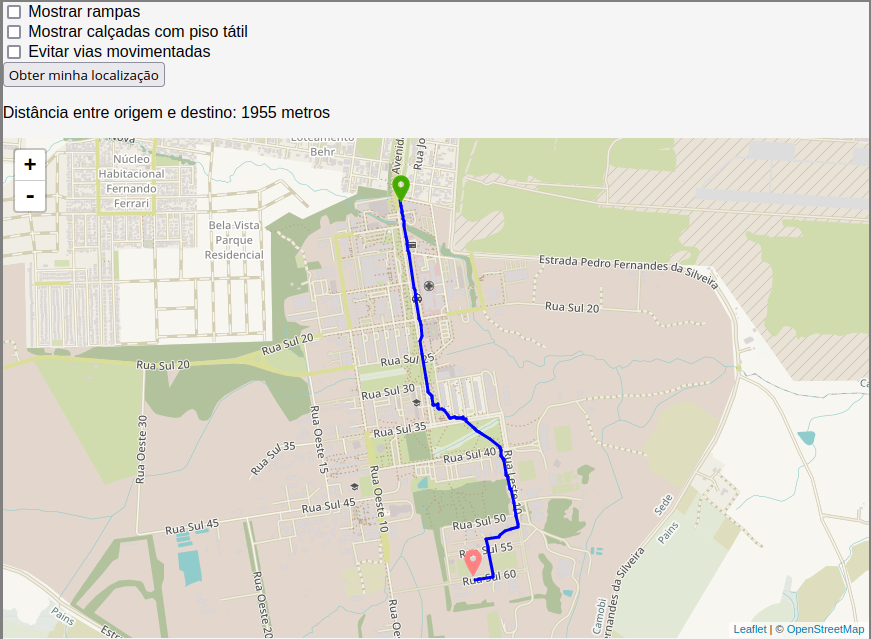
\includegraphics[scale=0.35]{imagens/arco-ce.png}}
 \quad
\subfigure[Resultado do Google Maps]{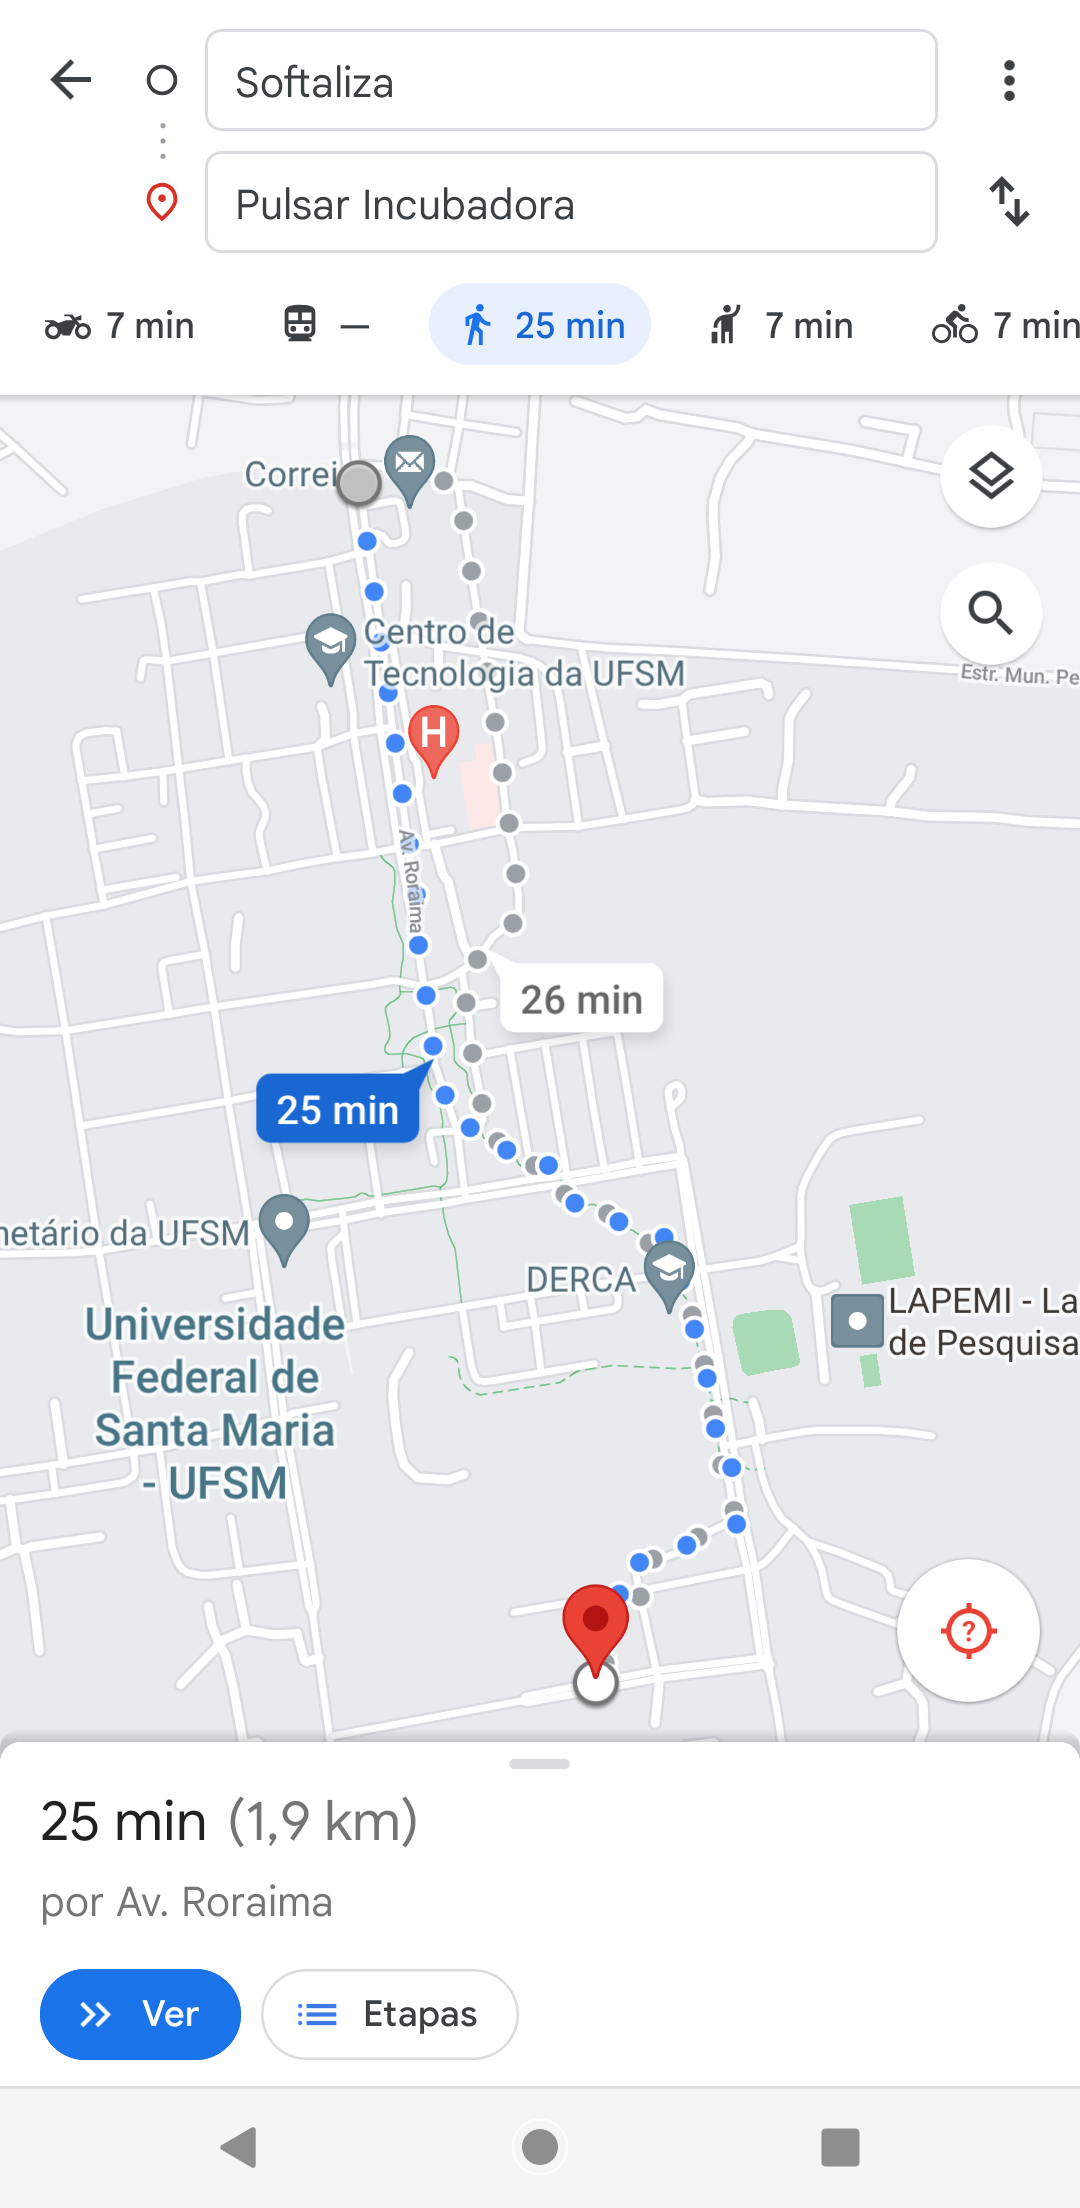
\includegraphics[width=0.35\textwidth]{imagens/arco-ce-gmaps.png}}
\quad
\subfigure[Resultado do OsmAnd]{ 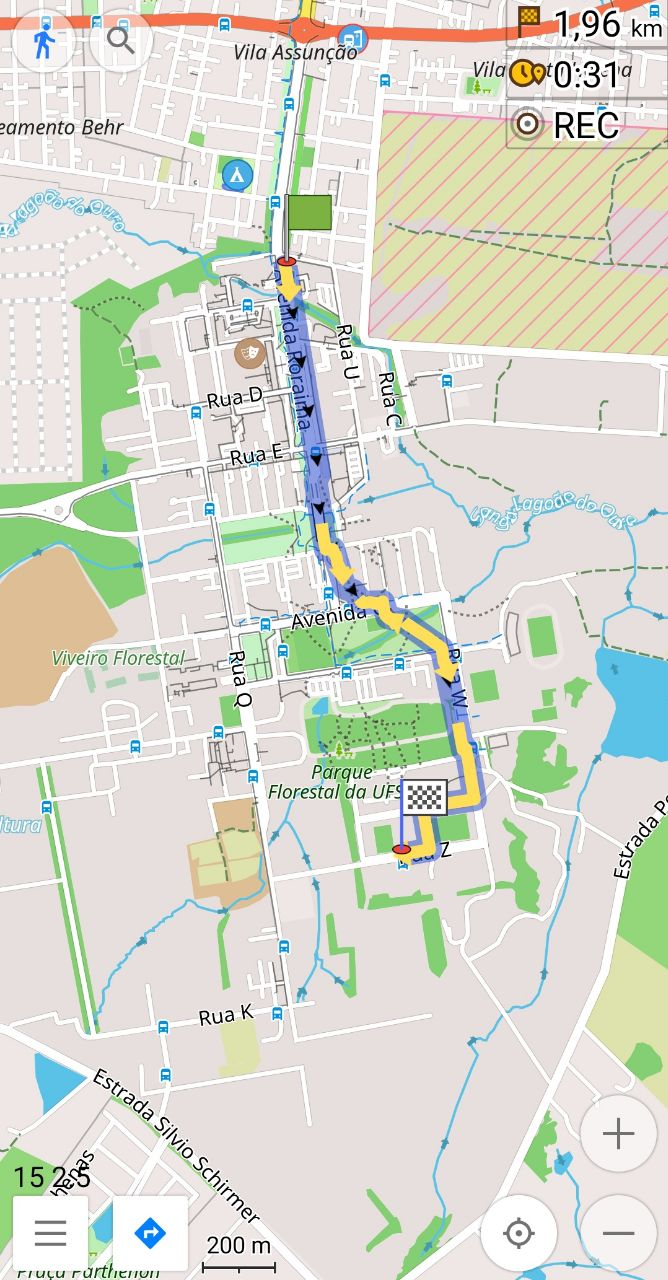
\includegraphics[width=0.37\textwidth]{imagens/arco-ce-osmand.jpeg}}
\label{fig:resultado_cenario1}
\fonte{(a) Próprio autor; (b) e (c) adaptado de aplicativos Google Maps e OsmAnd}
\end{figure}

\section{Caso de uso: Cenário 2} 
O Cenário 2 tem como ponto de origem a entrada do Departamento de Fitotecnia da UFSM e como ponto de destino o Restaurante Universitário I.
A Figura \ref{fig:resultado_cenario2}(a) apresenta o resultado da consulta na aplicação desenvolvida.
A Figura \ref{fig:resultado_cenario2}(b) apresenta o resultado da mesma consulta para o Google Maps e a Figura~\ref{fig:resultado_cenario2}(c) para o OsmAnd.

Os resultados da aplicação construída e dos resultados dos aplicativos são semelhantes na distância do trajeto, os três apresentando 1,2 km entre origem e destino. 
Entretanto, a aplicação desenvolvida e o OsmAnd sugerem um caminho por baixo da ponte da universidade, eliminando a necessidade de travessia pela Avenida Roraima, onde pode ser uma tarefa difícil cruzar de um lado até o outro devido ao intenso fluxo de veículos. 
O trajeto sugerido pelo Google Maps é semelhante até o Planetário da UFSM, mas logo depois sugere um trajeto pelas vias mais movimentadas da universidade. Esse aspecto da aplicação desenvolvida pode ser justificado pelo custo maior atribuído às vias da universidade com maior fluxo de veículos.

Nenhum problema de travessia foi alertado pela aplicação desenvolvida, porém é importante que seja mencionado o extenso trecho em que a rota sugerida passa pela via de veículos e não a calçada, entre o Departamento de Fitotecnia e o Politécnico, devido a um possível deficit de rampas mapeadas e/ou instaladas nesta área.



\begin{figure}[h]
\caption{Resultados de aplicativos de navegação para o cenário 2}
\centering
\subfigure[Resultado para a  aplicação]{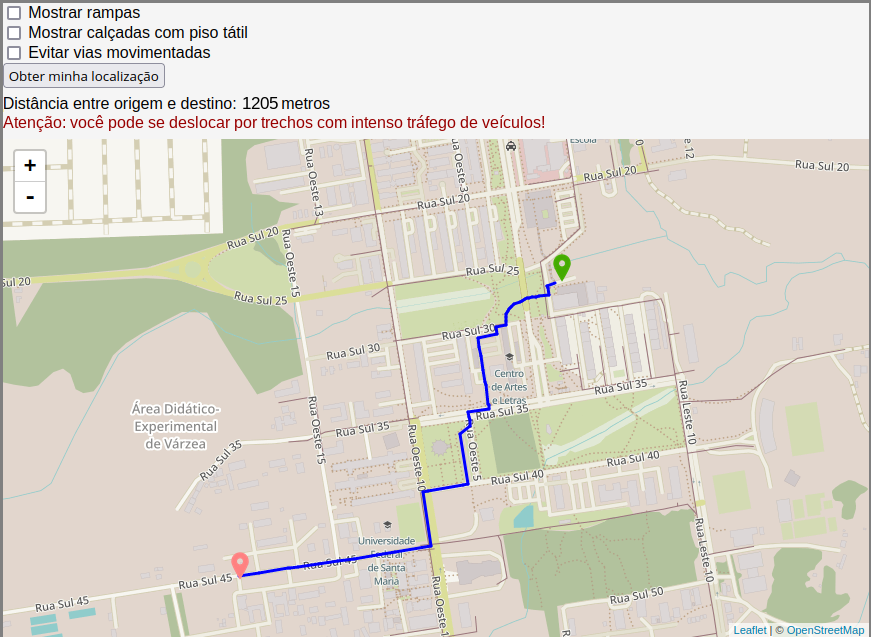
\includegraphics[scale=0.35]{imagens/fito-ru.png}}
\quad
\subfigure[Resultado do Google Maps]{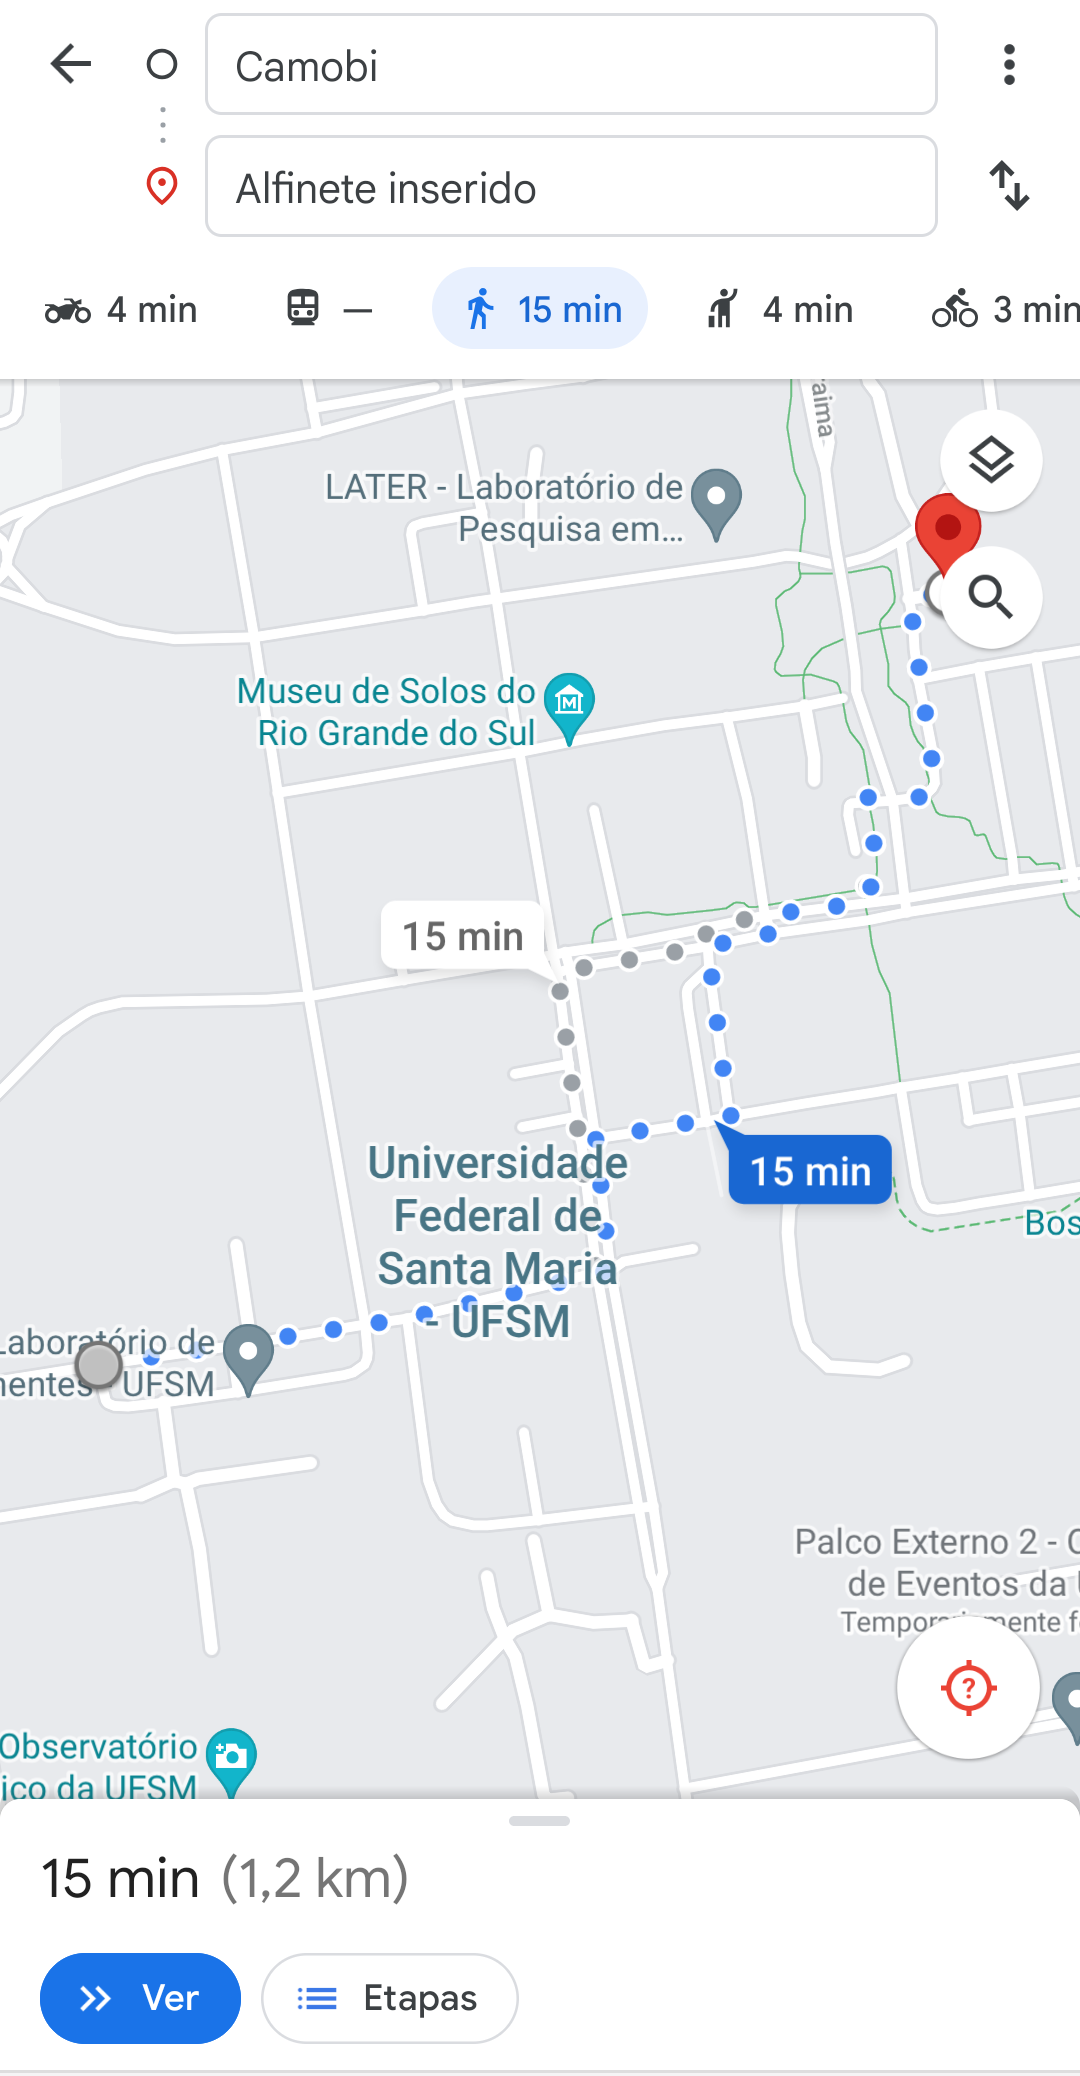
\includegraphics[width=0.35\textwidth]{imagens/fito-ru-gmaps.png}}
\quad
\subfigure[Resultado do OsmAnd]{ 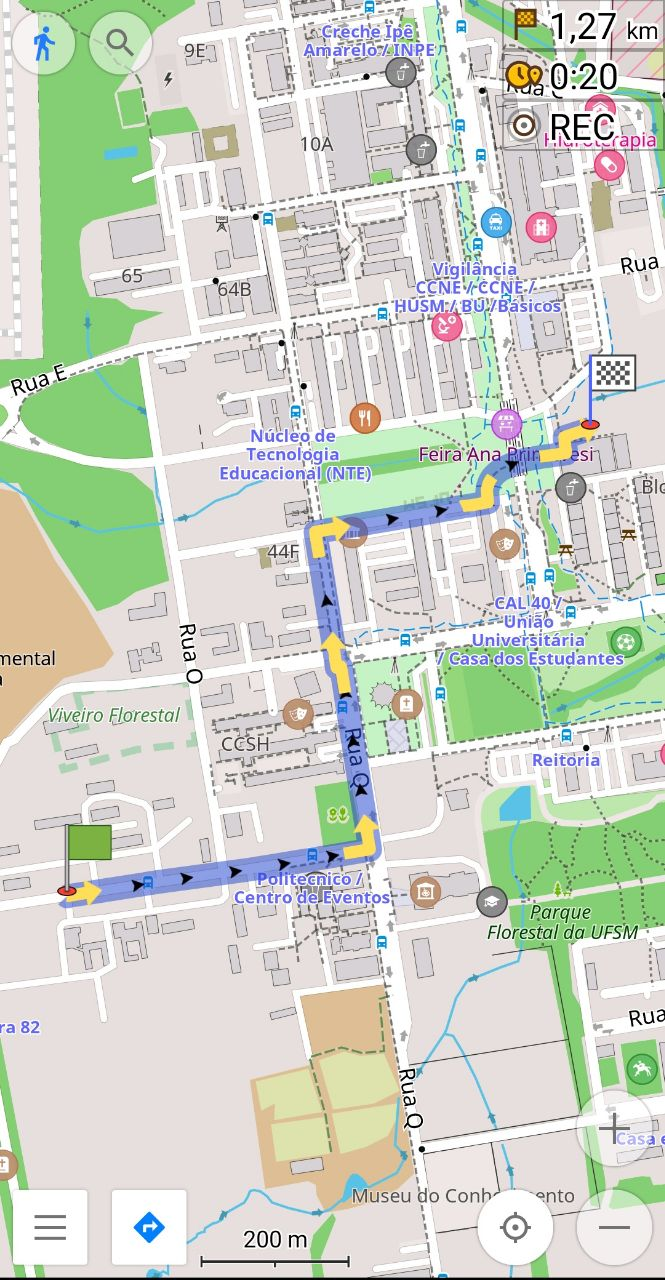
\includegraphics[width=0.38\textwidth]{imagens/fito-ru-osmand.jpeg}}
\fonte{(a) Próprio autor; (b) e (c) adaptado de aplicativos Google Maps e OsmAnd}
\label{fig:resultado_cenario2}
\end{figure}

\section{Caso de uso: Cenário 3}
O Cenário 3 tem como ponto de origem a entrada do Jardim Botânico da UFSM e como ponto de destino o Centro de Educação Física e Desportos da UFSM.
A Figura \ref{fig:resultado_cenario3}(a) apresenta o resultado da consulta na aplicação desenvolvida.
A Figura \ref{fig:resultado_cenario3}(b) apresenta o resultado da mesma consulta para o Google Maps e a Figura~\ref{fig:resultado_cenario3}(c) para o OsmAnd.
Os resultados da aplicação desenvolvida e os resultados do OsmAnd são semelhantes em distância e trajeto, com a aplicação desenvolvida e o OsmAnd mostrando um caminho de 2,15 km. 
O Maps mostra um caminho aproximadamente 50 m maior. 
A rota sugerida pela aplicação segue longitudinalmente até encontrar a ciclovia, que em praticamente todos os seus pontos de travessia com ruas, possui rampas de acesso, permitindo assim um deslocamento com maior autonomia. 
É importante ressaltar que do fim da calçada do Jardim Botânico até o encontro com a ciclovia, o trajeto é todo por via de veículos, já que neste trecho há pouca ou nenhuma disponibilidade de calçadas e rampas de acesso. 
Ainda assim, é uma via de menor tráfego.

\begin{figure}[h]
\caption{Resultados de aplicativos de navegação para o cenário 3}
\centering
\subfigure[Resultado para a aplicação]{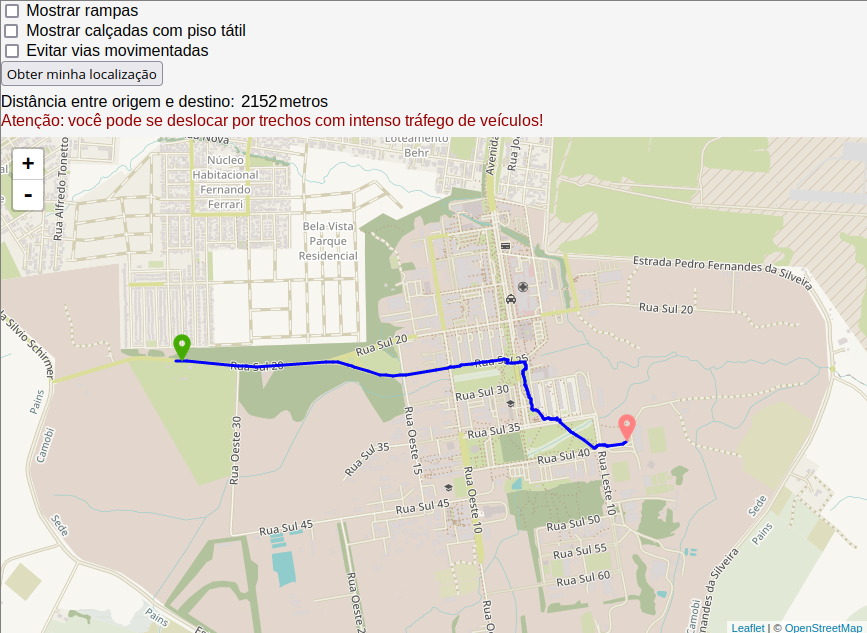
\includegraphics[scale=0.4]{imagens/jardim-cefd.png}}
\quad
\subfigure[Resultado do Google Maps]{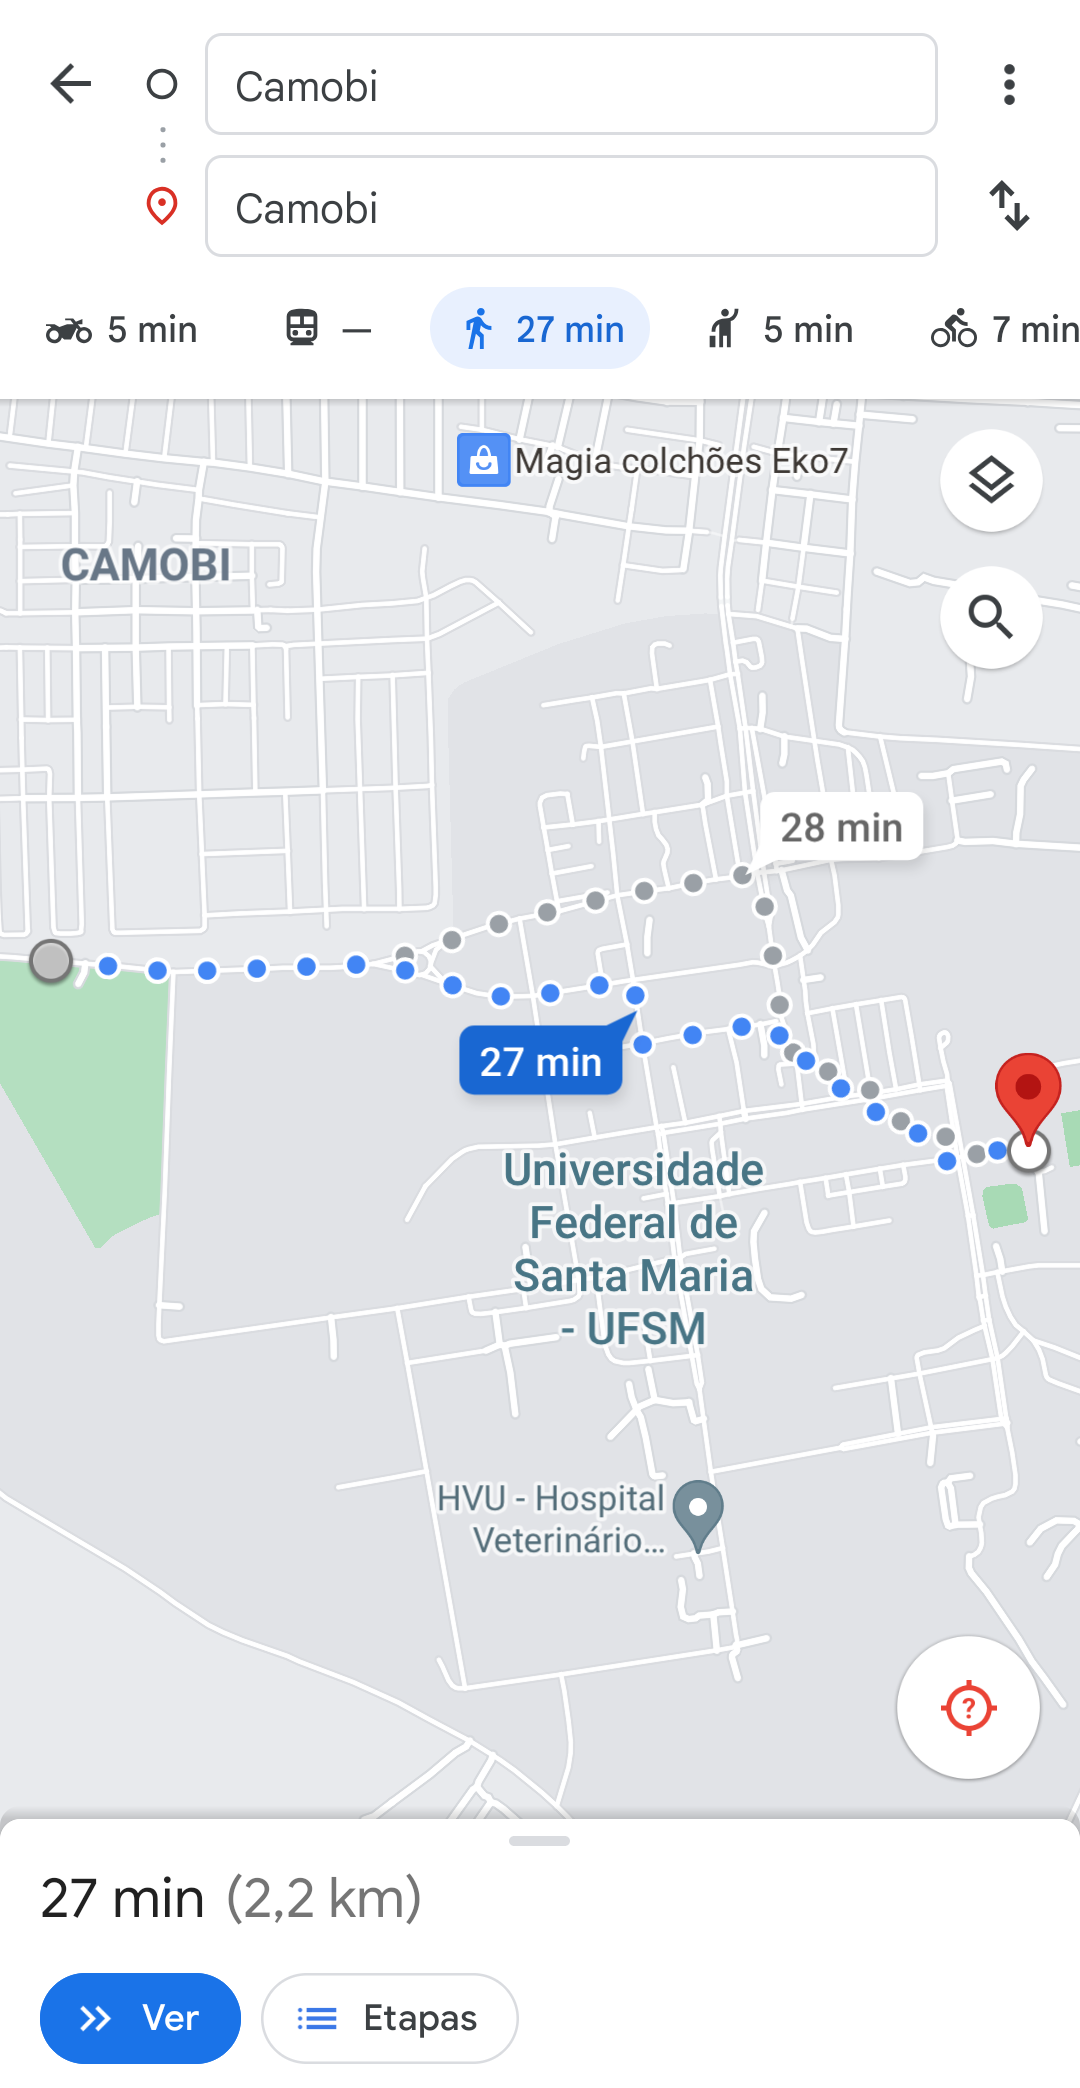
\includegraphics[width=0.3\textwidth]{imagens/jardim-cefd-gmaps.png}}
\quad
\subfigure[Resultado do OsmAnd]{ 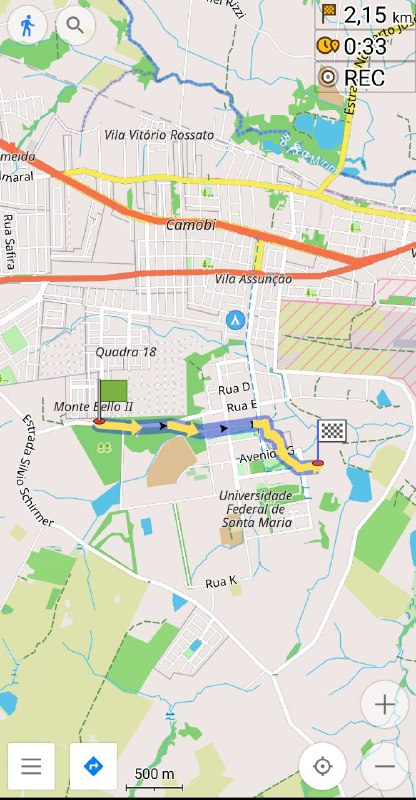
\includegraphics[width=0.3\textwidth]{imagens/jardim-cefd-osmand.jpeg}}
\fonte{(a) Próprio autor; (b) e (c) adaptado de aplicativos Google Maps e OsmAnd}
\label{fig:resultado_cenario3}
\end{figure}

\section{Caso de uso: Cenário 4}
O caso de uso 4 não aborda a consulta a rotas, mas a localização de rampas e pisos táteis dentro do campus Sede da UFSM. 
A Figura \ref{fig:rampas_mapa} mostra a localização de todas as rampas de acesso a calçadas da universidade, onde é possível perceber o submapeamento destas instalações na porção central e leste, privilegiando um conjunto de vias específicas com registro de rampa(s) a cada esquina. 
Não foi feita a comparação por \textit{ screenshots} porque nem Google Maps nem OsmAnd possuem uma função dedicada para visualizar no mapa localização de instalações de acessibilidade em calçadas.
\begin{figure}[h!]
    \caption{Localização de rampas de acesso a calçadas no campus Sede da UFSM}
    \centering
    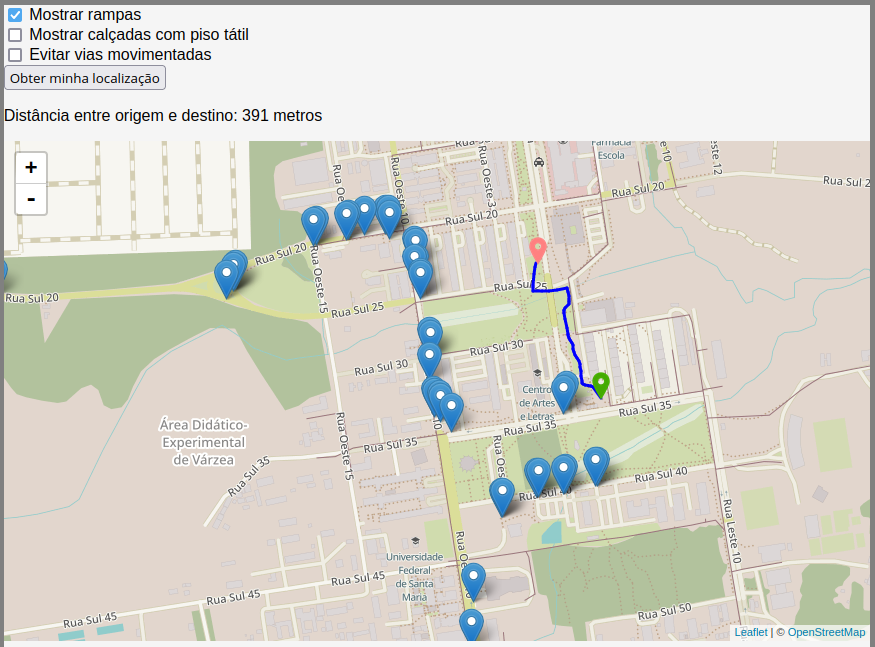
\includegraphics[scale=0.4]{imagens/rampas_mapa.png}
    \fonte{Próprio autor.}
    \label{fig:rampas_mapa}
\end{figure}


%--------------------------------------------------------------------------------------- 

% F - resultados pretendidos e indicadores
\chapter{Conclusões}
\label{sec:conclusoes}

Com o desenvolvimento da aplicação com a arquitetura proposta, foi demonstrada a potencialidade de uma base de dados geográfica colaborativa como fonte para soluções computacionais que tenham o espaço físico de um campus de universidade. Os resultados obtidos mostram que uma aplicação de cálculo de rotas para pedestres desenvolvida com dados e \textit{software} livre tem a capacidade de alcançar desempenho semelhante e em alguns casos até melhor do que soluções de aplicativos, bases cartográficas e APIs proprietários de grandes empresas de geotecnologias.

Além dos resultados obtidos em cálculo de rotas e visualização de instalações, é interessante avaliar a arquitetura do ponto de vista da inclusão de profissionais de outras áreas da universidade na manutenção da base, possibilitando que mapeamentos de rampas, pisos táteis e várias outras instalações realizados pelos setores de arquitetura, geoprocessamento e engenharia da universidade sejam atualizados e verificados por estes mesmos profissionais sem o intermédio de outro profissional, este com experiência em linguagem de consulta estruturada.

O principal problema identificado foi a utilização de apenas uma fonte de dados para a criação do banco de dados geográfico. Por mais que o mapeamento da universidade no OSM seja mais rico em número de elementos e metadados associados do que outras bases disponíveis, ainda assim, é possível observar que a ausência de alguns dados ou o submapeamento de algumas regiões comparadas a outras, levando a potenciais distorções na representação da realidade e no caso específico deste trabalho, sugestão de rotas inadequadas para pessoas com mobilidade reduzida. Uma ou mais fontes de dados com mapeamento completo do sistema viário da universidade é fundamental para sugerir rotas seguras fora da via para veículos e que priorizem rampas e faixas de pedestres. Por este motivo, é importante a combinação da base do OSM com uma base cartográfica oficial da universidade.

Os trabalhos subsequentes a proposta de arquitetura neste trabalho concentram-se principalmente em automação de importação e tratamento de dados, evolução do serviço fornecido pela API e refinamento de custos da rede criada. A automação permitirá que a atualização de dados no banco seja automaticamente refletida no cálculo de rotas, o que se mostra útil em caso de notificação de acidentes ou obstruções em vias, direcionando usuários por trajetos que não passem por estes segmentos intransitáveis.

A evolução dos serviços prestados pela API é importante pois neste trabalho, os serviços oferecidos se concentram em rotas no sistema viário da universidade e instalações de acessibilidade em calçadas, mas podem ser estendidos a estacionamentos, informando a quantidade de vagas para deficientes físicos e a prédios, informando quantos são e quais são os andares, banheiros e salas de aula acessíveis.

O refinamento de custos da rede é um trabalho multidisciplinar que deve ser acordado entre as diversas áreas de conhecimento onde há pesquisa sobre mobilidade urbana. Uma atribuição de custo baseada na hierarquia viária, a exemplo de uma avenida com maior custo de deslocamento do que o custo de uma calçada, retorna bons resultados, mas pode ser melhorada com base em outros fatores como declividade do terreno, superfície da via e até mesmo agradabilidade visual do percurso.

Além de atributos estáticos de variação temporal baixa, é importante também considerar o cálculo de custos sobre atributos dinâmicos, como aqueles obtidos por sensores conectados a rede da USFM ou através de inteligência coletiva por meio de usuários. A quantidade de pessoas circulando na via pode ser verificada por sensores, atualizando o banco de dados e criando polígonos a serem evitados para promover o distanciamento social recomendado pela OMS no contexto (pós-)pandemia. O nível de periculosidade de uma via pode ser atualizado por meio da submissão de informações por usuários de um  aplicativo que é conectado ao banco de dados, fazendo assim que rotas sugeridas evitem a região do evento suspeito.

Espera-se que este trabalho sirva como referência para a discussão de uma política de gestão de dados territoriais da universidade, utilizando \textit{software} livre e fontes de dados diversas, com o objetivo de construir uma fonte de consulta confiável e eficiente para usuários de instalações do campus.

%---------------------------------------------------------------------------------------
	
% % % % % % % % % % % % % % % % % % % % % % % % % % % % % % % % % % % % % % 
% % % % % % % % % % % % FIM DAS PAGINAS TEXTUAIS % % % % % % % % % % % % % % 
% % % % % % % % % % % % % % % % % % % % % % % % % % % % % % % % % % % % % % 



% % % % % % % % % % % % % % % % % % % % % % % % % % % % % % % % % % % % % % 	
% % % % % % % % % % % % % BIBLIOGRAFIA  % % % % % % % % % % % % % % % % % % 
% % % % % % % % % % % % % % % % % % % % % % % % % % % % % % % % % % % % % % 	

\bibliografia{biblio.bib}  %%%%% BIBLIOGRAFIA -> INCLUIR NAS CHAVES O NOME DO ARQUIVO *.BIB	
\end{document}\subsection{pgRouting}

